%%%%%%%%%%%%%%%%%%%%%%%%%%  phdsymp_sample2e.tex %%%%%%%%%%%%%%%%%%%%%%%%%%%%%%
%% changes for phdsymp.cls marked with !PN
%% except all occ. of phdsymp.sty changed phdsymp.cls
%%%%%%%%%%                                                       %%%%%%%%%%%%%
%%%%%%%%%%    More information: see the header of phdsymp.cls   %%%%%%%%%%%%%
%%%%%%%%%%                                                       %%%%%%%%%%%%%
%%%%%%%%%%%%%%%%%%%%%%%%%%%%%%%%%%%%%%%%%%%%%%%%%%%%%%%%%%%%%%%%%%%%%%%%%%%%%%%


%\documentclass[10pt]{phdsymp} %!PN
\documentclass[twocolumn]{phdsymp} %!PN
%\documentclass[12pt,draft]{phdsymp} %!PN
%\documentstyle[twocolumn]{phdsymp}
%\documentstyle[12pt,twoside,draft]{phdsymp}
%\documentstyle[9pt,twocolumn,technote,twoside]{phdsymp}

\usepackage[english]{babel}       % Voor nederlandstalige hyphenatie (woordsplitsing)

\usepackage{graphicx}			% Om figuren te verwerken.
\graphicspath{{../../../images/}}
\usepackage{booktabs}
\usepackage{times}
\usepackage{siunitx}
\usepackage{xcolor}
\usepackage{amsmath}
\PassOptionsToPackage{hyphens}{url}
\usepackage{hyperref}
\usepackage{url}

\usepackage[acronym,toc,shortcuts]{glossaries}
\setglossarystyle{super}
\renewcommand{\glsnamefont}[1]{\textbf{#1}}
\makeglossaries




%-------------------------------- acroniemen

\newacronym{UABS}{UABS}{Unmanned Arial Base Station}
\newacronym{EIRP}{EIRP}{equivalent isotropic radiation power}
\newacronym{UE}{UE}{User Equipment}
\newacronym{IEC}{IEC}{International Electrotechnical Commission}
\newacronym{SAR}{SAR}{Specific Absorption Rate}
\newacronym{whipp}{WHIPP}{WiCa Heuristic Indoor Propagation Prediction}
\newacronym{DL}{DL}{downlink}
\newacronym{UL}{UL}{uplink}
\newacronym{LTE}{LTE}{Long-Term Evolution}
\newacronym{FDD}{FDD}{Frequency Division Duplex}
\newacronym{TDD}{TDD}{Time Division Duplex}
\newacronym{ICNIRP}{ICNIRP}{International Commission on Non-Ionizing Radiation Protection}
\newacronym{LOS}{LOS}{line of sight}
\newacronym{NLOS}{NLOS}{non line of sight}
\newacronym{Exp Opt}{Exp. Opt.}{exposure optimized}
\newacronym{PwrC Opt}{PwrC. Opt.}{power consuption optimized}
\newacronym{WHO}{WHO}{World Health Organization}
\newacronym{FCC}{FCC}{Federal Communications Commission}
\newacronym{USA}{USA}{United States of America}
\newacronym{IOT}{IoT}{Internet of Things}
\newacronym{UAV}{UAV}{Unmanned Aerial Vehicle}
\newacronym{EU}{EU}{European Union}
%--------------------------------- woordenlijst
\newglossaryentry{isotropicradiator}{
	name = equivalent isotropic radiator,
	text = equivalent isotropic radiator,
	description = A theoretical source of electromagnetic waves which radiates the same intensity for all directions
}

\newglossaryentry{spuriousradiation}{
	name = spurious radiation,
	text = spurious radiation,
	description = According to the thefreedictionary.com: Any emission from a radio transmitter at frequencies outside its frequency band. Also known as spurious emission
}

\newglossaryentry{RRP}{
	name = RRP,
	text = RRP,
	description = RRP is an abreviation used in this paper to indicate an extension on EIRP and stands for Real Radiation Pattern. An RRP value indicates the power (in dBm) for a certain location unlike an EIRP where the power (in dBm) is independent of the location
}

\newglossaryentry{power flux density}{
	name = power flux density,
	text = power flux density,
	description = Magnitude of power ($W$) that travels through a curtain area ($m^2$)
}

\newglossaryentry{thermoregulatory capacity}{
	name = thermoregulatory capacity,
	text = thermoregulatory capacity,
	description = The capacity of an organism to regulate body temperture
}

%\printglossary[type=\acronymtype,title={Lijst van acroniemen}]
%\addcontentsline{toc}{chapter}{\textcolor{maincolor}{Lijst van acroniemen}}
%\printglossary
%\addcontentsline{toc}{chapter}{\textcolor{maincolor}{Verklarende woordenlijst}}






\hyphenation{si-mu-la-ted re-a-lis-tic packets really in-clu-ding}

\def\BibTeX{{\rm B\kern-.05em{\sc i\kern-.025em b}\kern-.08em
    T\kern-.1667em\lower.7ex\hbox{E}\kern-.125emX}}

\newtheorem{theorem}{Theorem}

\begin{document}
\title{Evaluating Human Electromagnetic Exposure in a \gls{UAV}-aided Network}

\author{Thomas Detemmerman}

\supervisor{Prof. dr. ir. Wout Joseph, Prof. dr. ir. Luc Martens} %Dr. ir. Margot Deruyck, Mphil. German Dario Castellanos Tache

\maketitle

\begin{abstract}
Society relies more than ever on the availability of wireless networks.
Due to the mobility of a UAV, a UAV-aided network is able to provide this necessary access in case the existing terrestrial network gets damaged.
However,  the public is 
concerned about the potential health effects of the electromagnetic radiation caused by these networks.
Therefore, mobile devices and base stations have to comply to strict legislation enforced by the government.

This research investigates how different scenarios influence power consumption, electromagnetic exposure and specific absorption rate.
These different scenarios are defined by various flying heights, number of UAVs available and population densities. Further, also 
an analysis on the difference
between a realistic microstrip patch antenna and a fictional equivalent isotropic radiator is performed.
Thereafter, the network will be optimized towards goals like electromagnetic exposure of the average user or 
power consumption of the entire network; which results in conflicting requirements.

To accomplish this goal, a capacity based deployment tool will be used which simulates an entire UAV-aided network.
In this way, all important sources for electromagnetic radiation, like all user equipment and all flying base stations, 
will be considered.

It looks from the results that a power consumption optimized network with a fixed flying height of 80 metres is the recommended approach
for the city centre of Ghent.
A microstrip patch 
antenna with a sufficiently large aperture angle is a good starting point. However, different antenna array configurations still have to 
be investigated.
\end{abstract}

\begin{keywords}
LTE, microstrip patch antenna, radiation pattern, specific absorption rate (SAR),
deployment tool, electromagnetic exposure, power consumption, wireless access network, 
emergency network, UAV, unmanned aerial base stations
\end{keywords}

\section{Introduction}
\PARstart{S}{ociety} is constantly getting more and more dependent on wireless communication. 
On any given moment, in any given location, an electronic device
can request to connect to the bigger network, 
starting from small \gls{IOT} up to self-driving cars.

Also in exceptional and possibly life threatening situations, the public relies on the cellular network
despite the fact that the network might be severely damaged and not properly functioning anymore.
One solution for a fast temporarily deployable back-up network is to use \gls{UAV}s. A base station can be attached to 
these flying \gls{UAV}s to support the network over a limited area. 
This approach is also useful in case of an unexpected increase in traffic. 
For example during the terrorist attacks at Brussels Airport,
mobile network operators saw all telecommunications drastically increasing causing moments of contention. 
Some operators even decided to temporarily exceed the exposure limits in
order to handle all connections \cite{baseZaventem}.
Electromagnetic exposure caused by these networks can however not be neglected. 
Research shows how excessive electromagnetic radiation can cause diverse biological side effects \cite{bioeffects,WHO}.
It becomes clear that electromagnetic exposure is a key value when designing a \gls{UAV}-aided network and should definitely 
not surpass the limits predefined by the government.

\gls{UAV}-aided networks can, thanks to their mobility, easily be repositioned towards a certain goal. Several papers 
explain how a network can be optimized towards different goals like power consumption.
However, very limited
research has been done where a \gls{UAV}-aided network is optimized towards electromagnetic exposure.
While several publications exist, discussing how the electromagnetic exposure can be calculated, 
most of them only consider a limited number of sources; e.g. only base stations or only the user's mobile device.
Papers who cover electromagnetic exposure from all the different sources and convert it into a single value are rather limited.

This research proposes a method to optimize the network towards electromagnetic exposure and power consumption
when considering all four sources of radiation in a telecommunications network, being: the user's own phone,
 the base station that is serving this user, 
all devices from other users in the network and all 
other active base stations that are not serving this user. In this way, the contribution of each source towards the total 
electromagnetic exposure can easily be identified. 

The behaviour of the electromagnetic exposure and power consumption of the network will be analysed
 by applying the tool in different scenarios by using different types of antennae, various flying height and population 
densities.
Values like \gls{SAR}, electromagnetic exposure and power consumption will 
 give insight in how the network behaves so the network could be optimized accordingly.

To make this research possible, 
an existing capacity based deployment tool developed by the WAVES research group at Ghent University is extended for the specific purpose.
This planning tool describes a fully configured \gls{UAV}-network which is a suitable starting point for this research.


\section{State of the Art}
\subsection{Electromagnetic exposure}

Users in a telecommunication network are exposed to various sources of electromagnetic radiation, expressed in $V/m$. Once the exposure is absorbed by the human 
body, we speak of the specific absorption rate (SAR) which is expressed in $W/kg$. All these values are 
subjected to limitations enforced by the government. This research is based in Ghent, 
a Flemish city in Belgium where the 2.6 GHz frequency band, an individual antenna cannot exceed 4.5 V/m and the cumulative sum of all 
fixed sources has its maximum at 31 V/m \cite{J23,S13_normenBelgie}. The maximum whole body SAR-values for a mobile device 
over a 10 g tissue ($SAR_{10g}$) is defined at $2 W/kg$ \cite{J30}. 

Several papers calculate exposure originating from specific sources  \cite{J6_originalExposureFormula,J1,J10_RDP,J10.1} 
where some convert the \gls{UL} radiation into localized specific absorption rates \cite{J10_RDP,J10.1}. 
With the advent of 5G, paper \cite{J17_kuehn2019modelling} describes 
how the localized \gls{SAR}-values are achieved from all different sources.
Finally, \cite{J22_plets2015joint} describes how the electronic radiation can be converted into whole body SAR values.

In a realistic network, some users are calling while others are using other types of telecommunication services like browsing the web.
Therefore, all absorbed electromagnetic exposure should be expressed in whole body SAR while still covering all sources.

\subsection{Optimized \gls{UAV}-aided networks}

A \gls{UAV} knows several applications. It was originally mainly used to support the military for surveillance and remote attacks without 
endangering pilots \cite{U12}. However, \gls{UAV}s have recently become more accessible by the general public due to decreasing costs. This 
allowed \gls{UAV}s to be researched for various applications.

A \gls{UAV} equipped with a femtocell base station antenna is called a \gls{UABS}
which brings several advantages like mobility and rapid deployment. 
However, it brings also challenges like limited weight of the payload and sparse power supply.

Kawamoto et al. introduced in \cite{U11} a WiFi network with the support of  \gls{UAV}s while considering resource allocation 
and antenna directivity. 
Gangula et al. illustrates in \cite{U10} how \gls{UAV}s can be used as a relay for \gls{LTE}
and
Zeng et al. proposes in  \cite{U12} a tutorial in 5G-and-beyond wireless systems where challenges like 
energy consumption, mobility and antenna direction are discussed. 
In \cite{J2}, Deruyck et al. designed  a capacity based deployment tool for UAV-aided emergency
networks for large-scale disaster scenarios where an ideal flying height of 100 m is suggested. This was expanded 
in \cite{U1} with a performance evaluation of the direct-link backhaul of this tool where a slightly lower 
flying height of 80 metres is recommended.


Mozaffari et al. provides in \cite{U3} guidelines on how to optimize and analyse \gls{UAV}s equipped for 
wireless communication equipment.
A research area that has been excessively studied is the location solution optimization problem where networks are 
designed in such a way that certain goals like minimal power consumption or shortest flying distance are achieved \cite{U6,U7,U8,U9}.
These optimizations can be done through different implementation methods like exact algorithms or machine learning \cite{U3,U5}.

Research where network is optimized towards electromagnetic exposure is rather limited.
Deruyck et al. discusses in \cite{J1} how a terrestrial network can be optimized towards either a minimal exposure or minimal power consumption of the entire network.
However, to the best of the author knowledge, no research has been done where a \gls{UABS}-network has been optimized towards electromagnetic exposure.

\subsection{Technologies}

For the deployment of the network, the more robust \gls{UAV} from \cite{J2} will be used (details in table \ref{table:defaultconf}) and will be operating in the 2.6 GHz 
bandwidth. Since the users are assumed to experience a constant electromagnetic exposure without interruptions, frequency division duplex is used.

% problem antennae on drones
The onboard antenna of the \gls{UAV} will act as the gateway between the UE and the backhaul network.
However, determining which antenna to use and how to position it, can be challenging.
The radiation pattern from the antenna can be influenced by the \gls{UAV} \cite{A1}.
Also the fact that the \gls{UAV} will hover above the user makes tradional 2D modelling insufficient.
A 3D-model which accounts for both elevation and azimuth directivity 
will be required \cite{U12}.

The easiest radiation pattern is a hypothetical isotropic radiator which radiates equally in all directions.
Antennae that radiate equal quantities for a certain plane are called omnidirectional antennae \cite{U12} and several 
\gls{UABS}s use antennae like monopoles, dipoles and wing antennae \cite{A4,A10,A11,A12}.
Another type of antennae are directional antennae which save energy by focussing the electromagnetic energy where it 
is needed. One type 
that has excessively been researched in various array-configurations is a microstrip patch antenna \cite{A5,A6,A8}.
These provide several advantages compared to traditional antennae \cite{J13_microstripadvantages,J14_antennadesign}
like lightweightness, low in cost causing them to be more aerodynamic. 

A basic microstrip antenna consists of a ground plane and
a radiating patch, both separated by a dielectric substrate. 
Several variations exist like microstrip patch antennae, microstrip slot antennae and printed dipole antennae which
all have similar characteristics \cite{J13_microstripadvantages,J14_antennadesign}. 
They all are thin, support dual frequency operation and they all have the disadvantage that 
they 
will transmit at frequencies outside the aimed band which is also known as
spurious radiation. The microstrip patch and slot antenna support both linear
and circular polarization while the printed dipole only supports linear polarization. 
Further, the fabrication of a microstrip patch antenna is considered to be the easiest 
of the considered patch antennae \cite{J13_microstripadvantages}. 



\section{Methodology}
\subsection{Electromagnetic Exposure}
\subsubsection{Total Electromagnetic Exposure}
The total whole body SAR ($SAR^{wb,total}_{10g}$) of a user can be calculated by a simple sum of individual SAR values from the different sources
and is based on \cite{J17_kuehn2019modelling}. This formula assumes that the users are holding their device next to their ear and therefore 
investigates localized \gls{SAR} for head and torso area.
However for this case, this would result into incorrect conclusions since 
the position of the device relative to the user is unknown. 
The position of the phone can be next to the head but also in front of the user.
The induced electromagnetic radiation will therefore be expressed in function of the entire body.

\begin{equation} 
\begin{aligned}
SAR^{wb,total}_{10g} = SAR^{wb,myUE}_{10g} +  SAR^{wb,myUABS}_{10g} \\
+ SAR^{wb,otherUE}_{10g} + SAR^{wb,otherUABSs}_{10g}
\end{aligned}
\label{eq:overallSARwb}
\end{equation}

The first parameter, $SAR^{wb,myUE}_{10g}$, indicates the absorbed electromagnetic radiation by the whole body originating from the user's own device. Despite that the 
\gls{UL} radiation is destined for the serving \gls{UABS}, a portion of that radiation is directly absorbed by its user, due to the omnidirectional nature of the mobile's antenna.
The second parameter, $SAR^{wb,myUABS}_{10g}$, represents the \gls{DL} radiation caused by the \gls{UABS} that is serving the user.
As the third parameter, we have the $SAR^{wb,otherUE}_{10g}$ which is radiation caused by other people's devices. The radiation of these devices is once again 
destined for a specific \gls{UABS} but again, a portion of that \gls{UL} radiation will also be absorbed by our user.
Finally, $SAR^{wb,otherUABSs}_{10g}$ represents the \gls{DL} radiation by the other \gls{UABS}s to which our user is exposed to but not served by.
An illustration is given in figure \ref{fig:networkIllustration}.
The green arrow stands for near-field radiation, the others represent far-field radiation.

\begin{figure}[h!]
\centering
  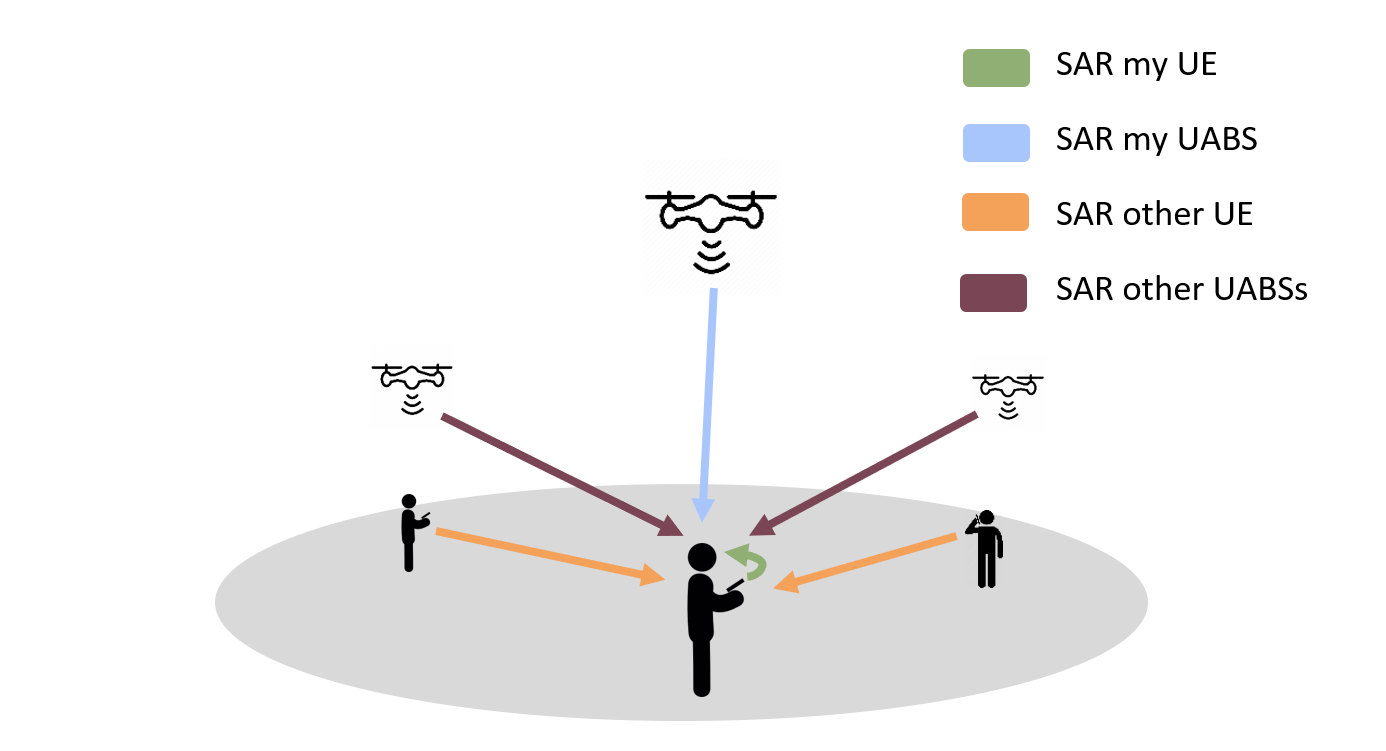
\includegraphics[width=\linewidth]{networkIllustrationSARSources.png}
  \caption{Illustration of the network that shows how the average user (here shown in the center) is influenced by different types of sources. }
  \label{fig:networkIllustration}
\end{figure}

\subsubsection{Electromagnetic Radiation from a Single Source}
\label{sec:calculatingexposure}

Calculating far-field exposure in a certain point needs to be done for all \gls{UABS}s and UE, except for the device 
present in that specific point which will be near-field radiation and has to be calculated differently.
The exposure $E$ of a single user $u$ from a single radiator $i$ can be calculated
as follows.

\begin{equation}
E_i(u) [V/m] = 10^{\frac{RRP(u)[dBm] - 43.15 + 20*\log(f [MHz])- PL(u) [dB]}{20}}
\label{eq:singleexposure}
\end{equation}

Calculating the real radiation power (RRP) for a certain user $u$, requires first the \gls{EIRP}-value to be calculated  \cite{J6_originalExposureFormula,J1}.
This is achieved by adding the transmission power $P_{tx}$ to the transmitter gain $G_t$ and thereafter subtracting the feeder loss $L_t$.
This formula needs to be expanded to also account for attenuation from the used antenna. This value depends on the angle
between this user and the antenna's main beam. The attenuation from an \gls{isotropicradiator} is always zero. This leads to the following formula.

\begin{equation}
\begin{aligned}
RRP [dBm] = P_{tx} [dBm] + G_t [dBi]- L_t [dB]\\
     - attenuation(u) [dB]
\end{aligned}
\label{eq:eirp}
\end{equation}
The used frequency in formula \ref{eq:singleexposure} is denoted as $f$ and is expressed in MHz. Since \gls{LTE} is used, this value will be 2600 MHz.

At last, formula \ref{eq:singleexposure} requires the path loss $PL$. In order to calculate this, an appropriate propagation model ---of which several exist--- is required.
The Walfish-Ikegami model is used since it performs well for femtocell networks in urban areas \cite{J2}. %optioneel kan je hier dezelfde bron gebruiken als dat ze in thesis van de vorige gebruikten. Bron nummer 32
%It consists of two formulas depending on whether a free LOS between the user and the base station exists or not. Both formulas expect a distance in kilometre. %bron?

\subsubsection{Combining Exposure}
The total electromagnetic exposure $E_{tot}$, in a certain spot, originating from different sources can be calculated with formula \ref{eq:totalexposure}. $E_i$ stands for 
the electromagnetic exposure from source $i$ and
$n$ stands for all far-field radiators of a certain category which will either be UABSs or UE from other people.
$E_{tot}$ will be calculated for each location where a user is positioned.  
\begin{equation}
E_{tot} [V/m] = \sqrt{\sum_{i=1}^{n} (E_i [V/m]) ^2}
\label{eq:totalexposure}
\end{equation}

\subsubsection{Converting electromagnetic radiation into SAR-values}

Formula \ref{eq:overallSARwb} expects that the radiation is expressed in whole body \gls{SAR}-values.
To make this calculation possible, a distinction has to be made between near-field \gls{SAR}
($SAR^{wb,nf}$) and far-field \gls{SAR} ($SAR^{wb,ff}$). $SAR^{wb,myUABS}_{10g}$ is a form of near-field radiation, 
all the other types are far-field radiation.
%$SAR^{wb,my\_UABS}_{10g}$, $SAR^{wb,other\_UE}_{10g}$ and $SAR^{wb,other\_UABSs}_{10g}$ are forms 
%of far-field radiation while $SAR^{wb,my\_UABS}_{10g}$ is a form of near-field radiation.

Converting the electromagnetic radiation is done with a conversion factor which is based 
on Duke of the Virtual Family. Duke is a 34-year old male with a weight of 72 kg, a height of 1.74 m and body
mass index of 23.1 kg/m \cite{J22_plets2015joint}. 
Research shows that the conversion factor for WiFi in the far-field is $0.0028 \frac{W/kg}{W/m^2}$
and 0.0070 $\frac{W/kg}{W}$ for the near-field \cite{J22_plets2015joint}.
Since WiFi, at a frequency of 2400 MHz,
is very close to \gls{LTE}, at 2600 MHz, it is assumed in \cite{J22_plets2015joint} that this value is also applicable for \gls{LTE}.
Calculating \gls{SAR} from far-field radiation is done as follows.

\begin{equation}
S [W/m^2]= \frac{(E_{tot} [V/m])^2}{337}
\label{eq:flux}
\end{equation}
\begin{equation}
SAR^{wb,ff}_{10g} [W/kg]= S [W/m^2]* 0.0028 \left[\frac{W/kg}{W/m^2}\right]
\label{eq:DLconversion}
\end{equation}

The constant in equation \ref{eq:DLconversion} converts the \gls{power flux density} $S$ to the required $SAR^{ff,wb}_{10g}$.
To make this possible, the electromagnetic radiation
from formula \ref{eq:totalexposure} should first be converted to the  \gls{power flux density} with formula 
\ref{eq:flux}.

The SAR caused by near-field radiation is calculated by multiplying the constant with the used transmission
power $P_{tx}$ of the \gls{UE} which results to the following formula.

\begin{equation} 
SAR^{wb,nf}_{10g} \left[\frac{W}{kg}\right] = 0.0070 \left[\frac{W/kg}{W}\right] * P_{tx} [W]
\label{eq:ulToSar}
\end{equation}

\subsection{Microstrip Patch antenna}
A microstrip patch antenna is chosen because it allows easy production but more important, it has a low weight 
and has a thin profile causing it to be very aerodynamic which is useful when attaching it to a drone \cite{J13_microstripadvantages}.

The dimensions of the antenna depend on the frequency it is operating at and the characteristics of the used substrate.
The antenna will be radiating at a centre frequency $f_0$ of 2.6 GHz. Each substrate has a dielectric constant $\epsilon_r$ representing 
the permittivity of the substrate that depends on the used material.
Substrates with a high dielectric constant and low height 
reduce the dimensions of the antenna
while a lower dielectric constant with a high height improves the performance of the antenna \cite{J14_antennadesign,J15_antennadesign}. 
In this research, a substrate like glass 
is chosen because of the higher dielectric constant of $\epsilon_r = 4.4$ compared to materials like Teflon with only a dielectric 
constant of $\epsilon_r = 2.2$ \cite{J14_antennadesign}. 
Doing this in combination with an antenna height of 2.87 mm will decrease the dimensions of the entire antenna surface.
This comes in handy since drones only have limited space available.

\begin{table}[h!]
\centering
\begin{tabular}{|l|c|l|}
\hline
 description            & symbol          & value         \\    \hline
 centre frequency       & $f_0$           & 2600 Hz       \\ 
 dielectric constant    & $\epsilon_r$    & 4.4         \\ 
 height of the substrate & $h$             & 0.00287 m    \\ \hline
\end{tabular}
\caption{Overview of configuration parameters.}
\label{table:antennaparas}
\end{table}

The dimensions of the radiating patch can be calculated with the formulas from \cite{J14_antennadesign,J15_antennadesign}.
Doing so will result in a radiating patch of 35.09 mm by 26.55 mm and a groundplane of at least 52.40 mm by 43.80 mm.
The microstrip patch antenna as illustrated in fig. \ref{fig:basicpatchantenna} will result in the radiation pattern of fig. \ref{fig:radpattern}.
\begin{figure}[h!]
\centering
  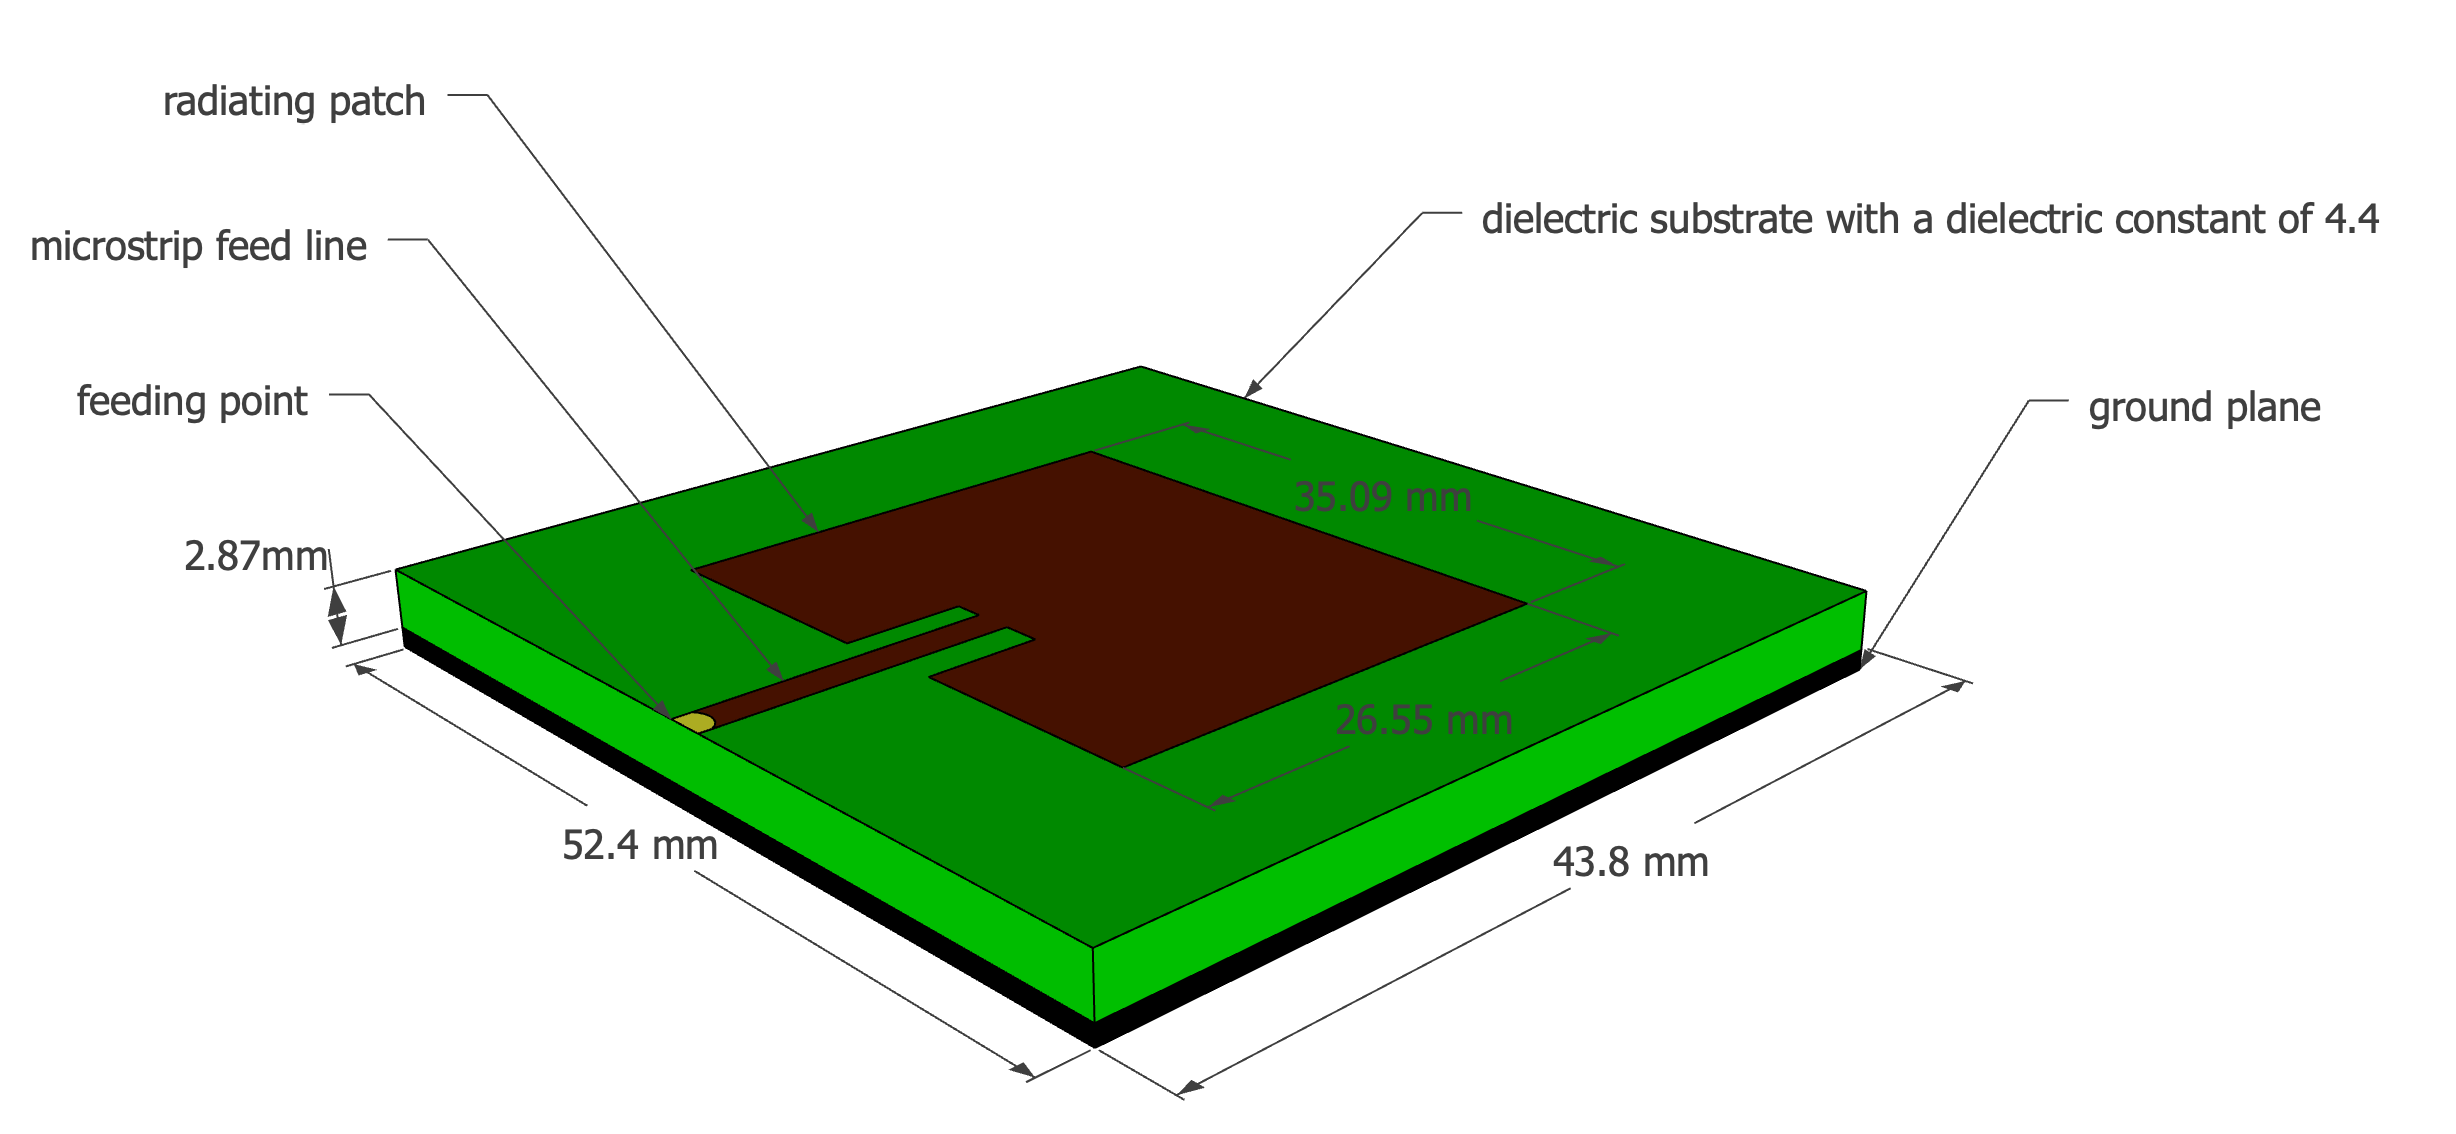
\includegraphics[width=\linewidth]{MicrostripAntenna.png}
  \caption{Design of the microstrip patch antenna.}
  \label{fig:basicpatchantenna}
\end{figure}


\begin{figure}[!htb]
\minipage{0.50\linewidth}
  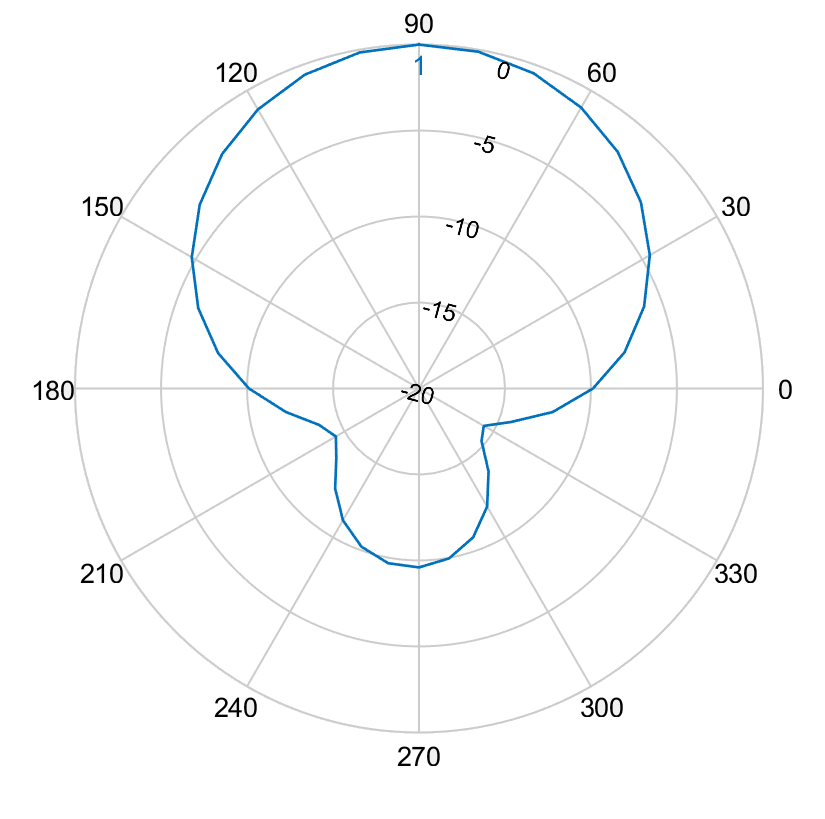
\includegraphics[width=\linewidth]{pattern2/ep.png} 
\endminipage\hfill
\minipage{0.50\linewidth}%
  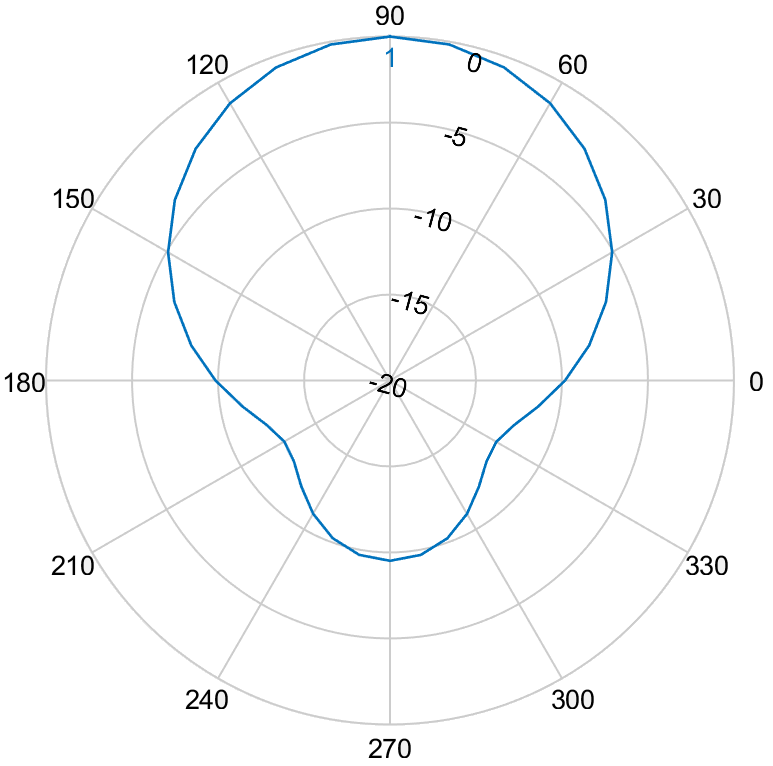
\includegraphics[width=\linewidth]{pattern2/hp.png}
\endminipage
  \caption{On the left is the radiation pattern of the E-plane drawn and on the right for the H-plane.}
\label{fig:radpattern}
\end{figure}

\subsection{Optimizing the network}

Deruyck et al. discusses in \cite{J1} how a terrestrial  telecommunication network either can be optimized towards electromagnetic 
exposure of an individual or towards power consumption of the entire network. 
However, an increasing transmission power of an antenna comes with an increasing electromagnetic exposure. This is not the case considering
both values for an entire network. In fact, the authors from \cite{J1}  prove that both become inversely equivalent.
The reason why the network behaves like this is because it is often cheaper to increase the exposure of an already active base station 
than activating a new one. 
This leads to the following fitness function which is based on \cite{J1}.

\begin{equation} 
f = w * \left(1 - \frac{E_m}{E_{max}}\right) + (1 - w)*\left(1 - \frac{P}{P_{max}}\right) * 100
\label{eq:fitnessfunction}
\end{equation}

Formula \ref{eq:fitnessfunction} returns a fitness value which represents the performance of the entire network. 
$w$ is the importance factor of electromagnetic exposure ranging from 0 to 1, boundaries included. A $w$ set to 0 means that electromagnetic 
exposure is not important. Such network will therefore be called a \gls{PwrC Opt} network. 
Likewise, a $w$ set to 1 means that minimizing exposure is top priority and will result in an \gls{Exp Opt} network. $P_{max}$ is the power consumption of all UABSs, 
both active and inactive, when radiating at the highest level possible 
while $P$ is the effective power used by the current designed network. 
This will be the power required for the flying drones themselves and their antennae.
$E_m$ will be the weighted exposure of the average user for the current designed network and $E_{max}$ the weighted average of the electromagnetic exposure when all antennae 
are at their highest power level.

When optimizing the network, it is not only important to consider the average exposure of all users, but also to limit high extremes \cite{J1}. A weighted average 
will be used not only considering the median but also the 95 percentile from all users' \gls{DL} exposure using formula \ref{eq:em}. 
Since both values are considered to have equal importance, the weight factors $w_1$ and $w_2$ will both have an equal importance of 50\%. 

\begin{equation} 
E_m = \frac{w_1 * E_{50} + w_2 * E_{95}}{w_1 + w_2}
\label{eq:em}
\end{equation}

\begin{figure}[h!]
  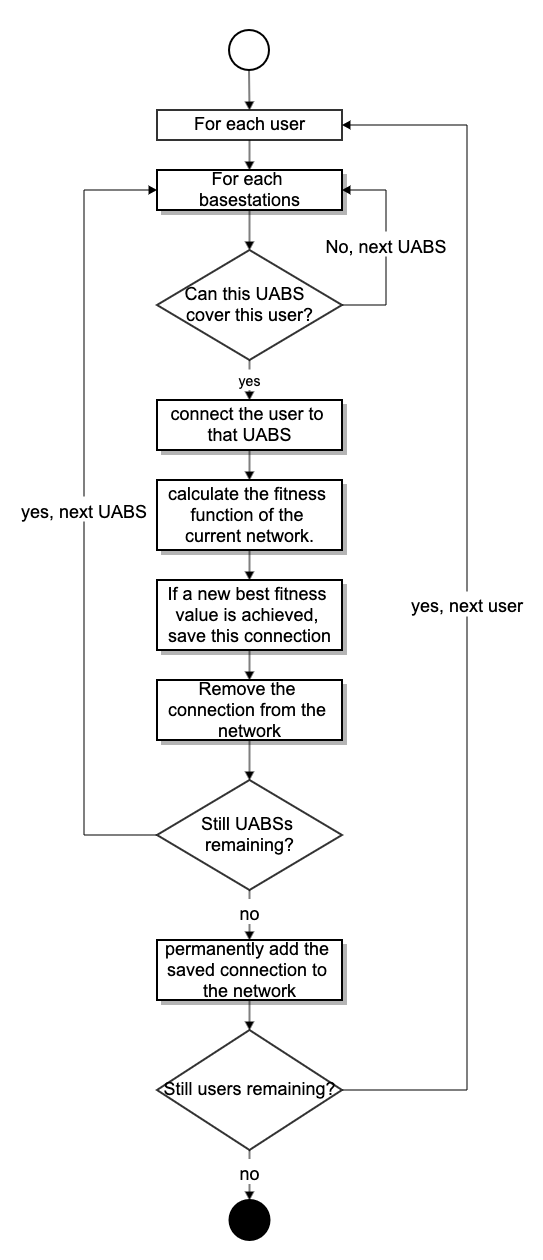
\includegraphics[height=0.8\textheight]{decisionAlgoFlowChart.png}
  \caption{Flowchart of the decision algorithm.}
  \label{fig:decisionAlgoFlowChart}
\end{figure}

\subsection{Simulation Tool}

\subsubsection{Main Algorithm}
First, a description of the area has to be provided to the tool. This is done with so-called shape-files.
These  files contain a complete description about the shape of the buildings. Thereafter, users are uniformly
distributed over the area and a temporary \gls{UABS} is positioned above each user. Now, the decision algorithm
needs to decide which of these \gls{UABS}s can actually remain and how hard each one should be radiating. Once the 
decision algorithm is done, the tool checks whether the number of online \gls{UABS}s does not acceed the capacity of 
the facility where the \gls{UABS}s are stored. If this is the case, the \gls{UABS}s covering the least amount of users 
will be removed.

\subsubsection{Decision Algorithm}

Solving the network is done by the decision algorithm and starts by calculating the path loss between all users and between users and \gls{UABS}s.
Thereafter, the algorithm iterates over each user and tries to connect that user to each \gls{UABS}. This connection is not always possible. A \gls{UABS} might be saturated with users and 
will not be able to cover yet another one or maybe the user is so far away that in order to cover that user, the \gls{UABS} would have to exceed its maximum allowed input power.
If however a connection is possible, the user will be connected to that \gls{UABS} and the fitness function (eq. \ref{eq:fitnessfunction} is applied. 
This is repeated for each \gls{UABS}. Only the connection which results in the best fitness value for the entire network will be used. Thereafter, the tool shifts to the next user. 
When the last user has been processed, the network is fully designed for an unlimited number of drones and the result is returned to the main algorithm for further processing.
The flowchart of this algorithm is given in figure \ref{fig:decisionAlgoFlowChart}.

%%%%%%%%%%%%%%%%%%%%%%%%%%%%%%%%%%%%%%%%%%%%%%%%%%%%%%%%%%%%%%%%%%%%%%%%%%%%%%%%%%%%%%%%%%%%%%%%%%%%%%%%%%%%%%%%%%%

\section{Scenarios}
The default configuration is given in table \ref{table:defaultconf} and is always applicable unless mentioned otherwise. 

\begin{table}[!htb]
\centering
\begin{tabular}[t]{ll}
        \toprule
        \multicolumn{2}{l}{\textbf{Broadband cellular network}} \\
        \hline
        \hspace{3mm}  technology        & LTE     \\
        \hspace{3mm}  frequency         & 2.6 GHz \\
        \hline
        \multicolumn{2}{l}{\textbf{UAV}} \\
        \hline  
        \hspace{3mm}  carrier power        & 13.0 A   \\
        \hspace{3mm}  average carrier speed        & 12.0 m/s \\
        \hspace{3mm}  average carrier power usage      & 17.33 Ah    \\
        \hspace{3mm}  carrier battery voltage       & 22.2 V \\
        \hline
        \multicolumn{2}{l}{\textbf{Femtocell antenna}} \\
        \hline  
        \hspace{3mm}  maximum $P_{tx}$          & 33 dBm   \\
        \hspace{3mm}  antenna  direction        & downwards   \\ 
        \hspace{3mm}                            & (az: \ang{0}; el: \ang{90})    \\
        \hspace{3mm}  gain                      & 4 dBm   \\ 
        \hspace{3mm}  feeder loss               & 2 dBm   \\ 
        \hspace{3mm}  implementation loss       & 0 dBm   \\
        \hspace{3mm}  radiation pattern         & EIRP or\\
         \hspace{3mm}                           & microstrip patch\\
        \hspace{3mm}  flying altitude           & 100m  \\
        \hline
        \multicolumn{2}{l}{\textbf{UE Antenna}} \\
        \hline 
        \hspace{3mm} height                     & 1.5m from the floor       \\ 
        \hspace{3mm} gain                      & 0 dBm   \\ 
        \hspace{3mm} feeder loss               & 0 dBm   \\ 
        \hspace{3mm} radiation pattern         & EIRP  \\
        \hspace{3mm} number present in the network         & 224  \\
        \toprule
\end{tabular}
\caption{Overview of default configuration values.}
\label{table:defaultconf}
\end{table}

Three main scenarios will be investigated. 
The first one has only one user and one \gls{UABS} present in the network. 
SAR, electromagnetic exposure, power consumption 
and antenna transmission power are investigated at different flying heights.

In a second scenario, the network is expanded for multiple users while still considering only one \gls{UABS}. 
The scenario is divided into two cases. One with a variable flying height but with a fixed 
number of 224 users as is average on an usual day at 5 p.m. in Ghent \cite{J2}.
 In the other case, the number of users varies but the flying height is set to 100 metres \cite{J2}.
The power consumption, electromagnetic exposure and specific 
absorption rate are investigated for each case.

The third scenario is quite similar to the previous scenario. The same two cases are investigated, but now an unlimited number of \gls{UABS}s is avalaible.

Each case from each scenario consists out of four possible configurations.
There are two possible antennae, namely EIRP 
and microstrip patch antenna, which can both be applied in a \gls{PwrC Opt} network or an \gls{Exp Opt} network.

It is important to note that 
all measured values are strictly limited to the sources mentioned in the previous section and thus only cover data traffic 
between \gls{UE} and \gls{UABS}s. Any other potential sources like backhaul links will not be covered.

An overview of the simulation configuration scenarios is presented in figure \ref{fig:fourCasesMatrix}

\begin{figure}[h!]
  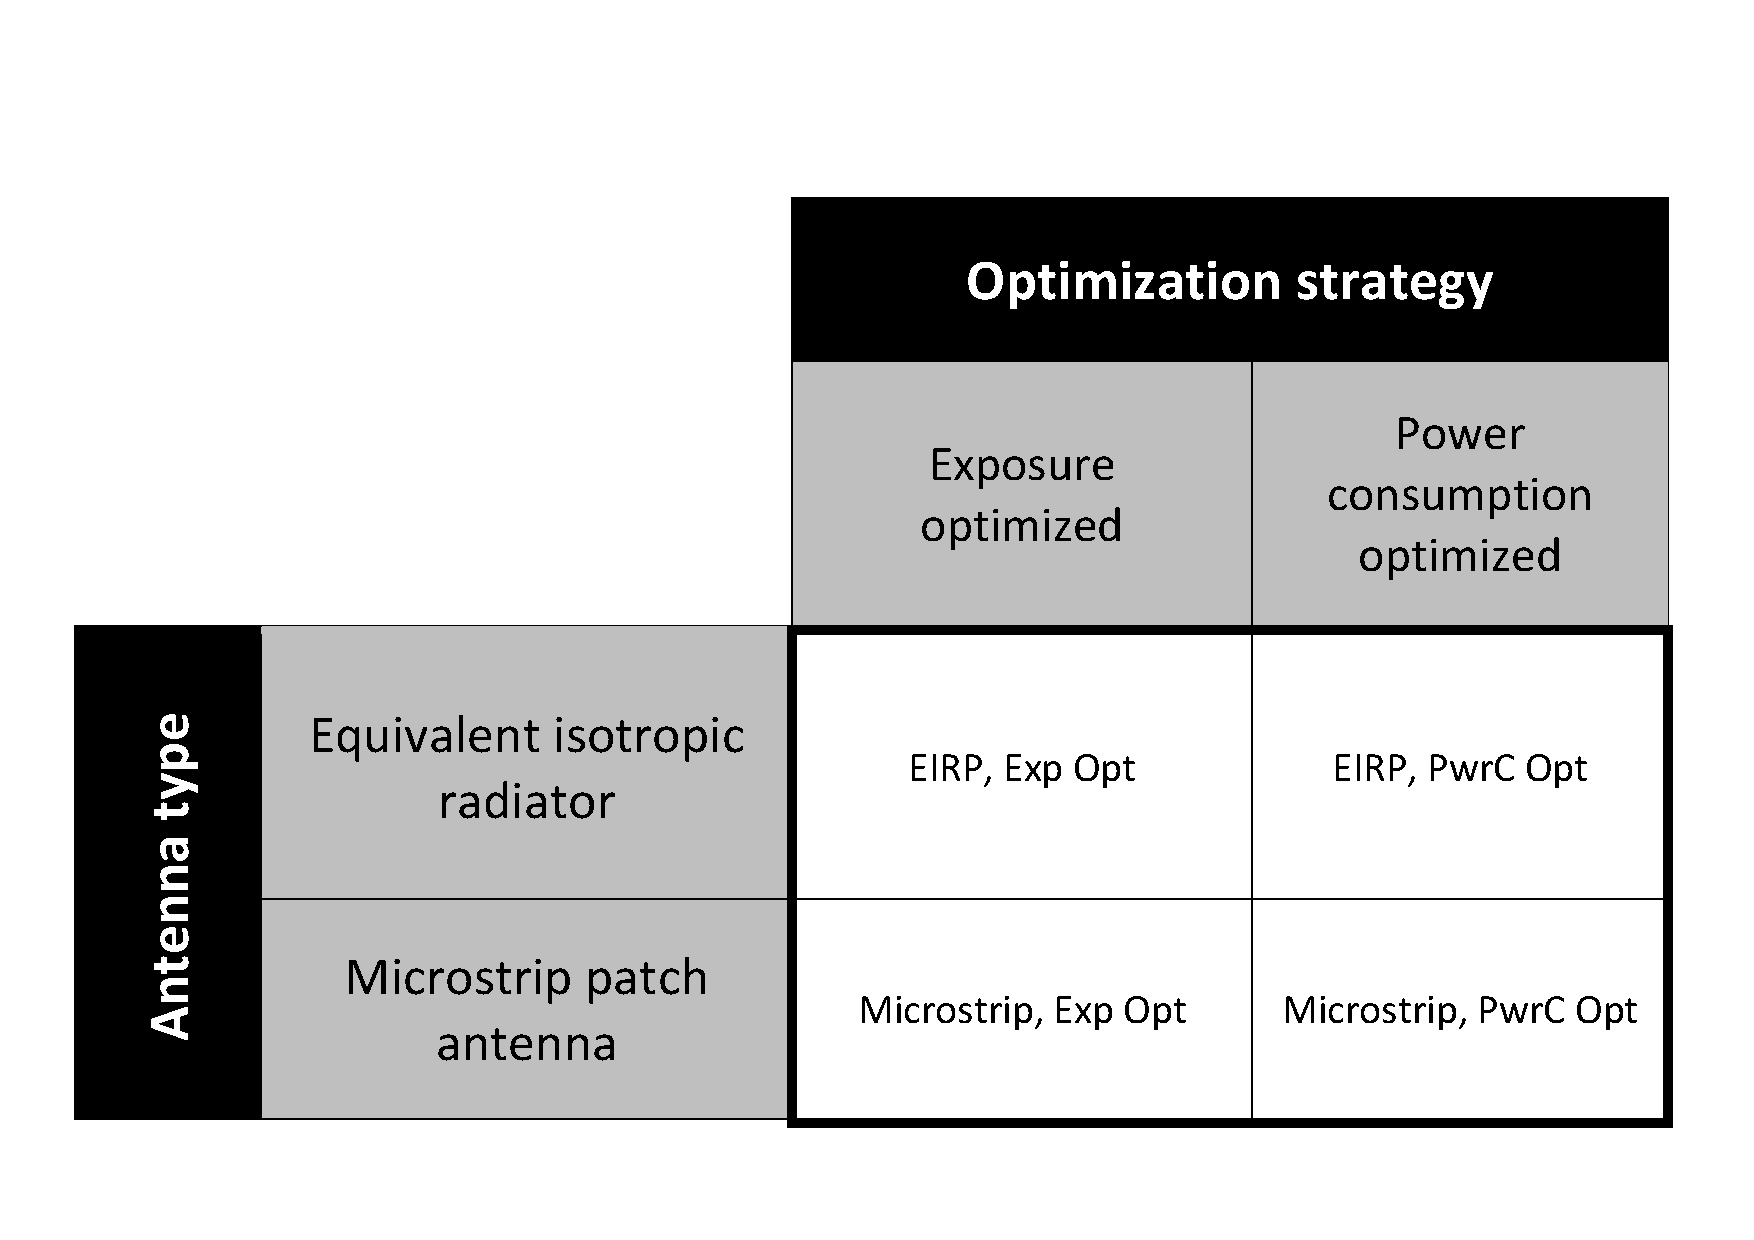
\includegraphics[width=\linewidth]{fourCasesMatrix.pdf}
  \caption{Matrix with the four possible configurations}
  \label{fig:fourCasesMatrix}
\end{figure}

\section{Results}
\subsection{One User and One \gls{UAV}}

The  results show that for a varying flying height, a logarithmic relationship exists between the $P_{tx}$ and the flying height. 
This is mainly caused by the logarithmic 
scale in which the decibels of the $P_{tx}$ are expressed. So while 10 dBm equals 10 mW, 20 dBm equals 100 mW. 
Each time the flying height becomes too large to cover, the 
$P_{tx}$ increases with one dBm. 
When using the default configuration, with a maximum $P_{tx}$ of 33 dBm,
a \gls{UABS} can fly up to 387 m before losing connection in a free \gls{LOS} scenario.

This scenario is investigated with a microstrip patch antenna using power consumption optimization. 
 However, the chosen optimization strategy does not really matter because the decision 
 algorithm decides which user 
needs to be connected to which \gls{UABS}. Since only one \gls{UABS} is available, both optimization strategies will behave identical.
Further, also the used antenna will not make any difference.
The user is namely positioned in the perfect centre of the main beam where there is 
no attenuation experienced for both antennae.

When investigating this scenario at different flying heights, we notice 
that the \gls{UL} radiation 
increases exponentially while 
the \gls{DL} radiation remains constant during the entire time. The reason that the \gls{DL} radiation
remains constant is because of power control which makes sure that no more power is used than strictly necessary. 
So at lower flying altitudes, there is less path loss and the \gls{UABS} 
will therefore reduce the $P_{tx}$. 
We can therefore confirm that the electromagnetic exposure is a constant fraction of power and distance.
The \gls{UL} radiation starts very low but surpasses the \gls{DL} radiation 
around 80 metres.
%\begin{equation}
%\vec{E} (V/m) = \frac{\Delta U (V) }{\Delta x (m)}
%\label{eq:exposureBasicFormula}
%\end{equation}

\subsection{Increased Population with one UABS}
\subsubsection{Variable Flying Height}
A \gls{PwrC Opt} network has higher exposure compared to an \gls{Exp Opt} network; a behaviour that was already proven by \cite{J1}. 
However, for this scenario, a \gls{PwrC Opt} network will also result in a higher power consumption. 
To understand this, the behaviour of the deployment tool needs to be understood first. 
A \gls{PwrC Opt} network will result in a few high powered \gls{UABS}s because increasing the input power of an antenna costs 
less than activating a new  \gls{UAV}. Likewise, an \gls{Exp Opt} network 
generates a lot of low powered \gls{UABS}s because the lower the power of the antenna, the lower the exposure. This has the consequence that the cover radius 
is less and therefore more UAVs, which cost more energy, are required.
When only a limited amount of \gls{UABS}s are available, 
like only one in this scenario, the tool will only keep \gls{UABS}s which cover the most users. 
Therefore, the power consumption in a \gls{PwrC Opt} network is much more higher. 

Further, the results also show that the exposure increases with higher flying altitudes
because there is a lower probability of having \gls{NLOS} links by obstructing buildings. This has as consequence that  
more users become covered. 
The increasing electromagnetic radiation is however not unlimited.
At even higher
flying altitudes, the distance between a given \gls{UABS} and some users further away becomes too large causing the 
coverage to decrease again. When this decrease occurs depends on the configuration. A \gls{PwrC Opt} 
network tends to decline earlier than an \gls{Exp Opt} network.

When replacing the fictional \gls{EIRP} antenna by a microstrip patch antenna, the percentage of covered users drops for both 
optimization strategies. This is because users, who have a higher horizontal distance between themselves and the \gls{UABS}, 
experience a higher attenuation.

The results further show  
that the radiation from the \gls{UABS} is the main factor followed by the near-field radiation from the user's own device.
The far-field radiation from other \gls{UE} barely contributes anything.

\subsubsection{Variable Number of Users}

Also the results from this case show how EIRP antennae designs are able to cover more users than microstrip patch antennae
just like \gls{PwrC Opt} networks will reach more users than \gls{Exp Opt} networks.
The contribution to the total \gls{SAR} from each individual source is identical to the previous scenario. 

There is still only one \gls{UABS} available. When population grows, more users become uncovered and 
therefore the average electromagnetic exposure decreases.
For example, an EIRP \gls{PwrC Opt} network
will have the highest exposure and therefore covers the most users as opposed to a microstrip patch antenna in 
an \gls{Exp Opt} network which will radiate the least and thus has the lowest number of covered users.

While the population grows, more and more users become uncovered causing the average SAR to drop. 
However, this does not conclude that by increasing the population, the SAR of a user who is directly beneath a \gls{UABS} would be less.
To investigate this, a user is positioned in the middle of the city centre of Ghent and a \gls{UAV} is positioned above him. Initially, only 
49 people are active around him. The \gls{SAR} of our central user is monitored while the population around him is growing.
Figure \ref{fig:connectionMap} shows with the black lines which users are connected. The left map is for only 50 users and 
shows that only one user is connected besides our central user. The map on the right considers 600 users and shows much more connected users.
The results show that the \gls{UL} \gls{SAR} of the central user remains constant; a normal behaviour since the flying altitude does not change.
The \gls{SAR} from the \gls{UABS} experiences a slight increase. When the population grows, more users become available 
and some will spawn near the central user. The \gls{UABS} will likely decide to cover these users as well as visible in figure \ref{fig:connectionMap}.
These users might have a slightly 
worse path loss because of obstructing buildings or a somewhat bigger distance. The \gls{UABS} reacts to this by increasing 
its power consumption causing an increase in the \gls{DL} \gls{SAR} for the central user. The results further also show 
that the \gls{SAR} from other \gls{UE} increases when the population increases. But as mentioned  before, it is much less 
compared to the other sources.

\begin{figure}[!htb]
\minipage{0.50\linewidth}
  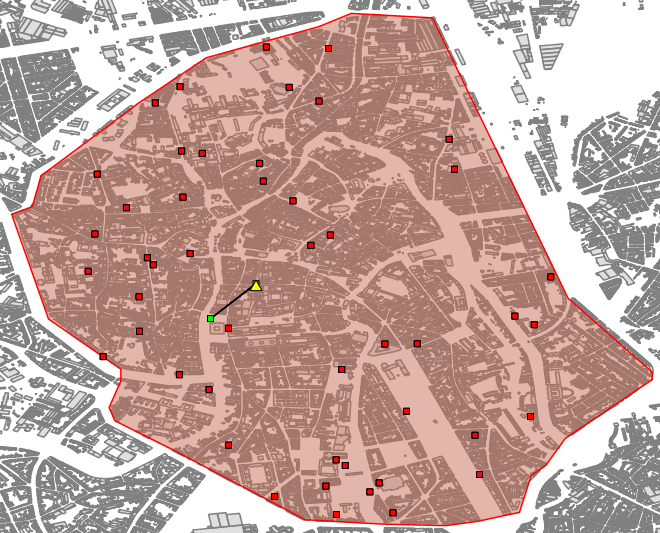
\includegraphics[width=\linewidth]{../images/connectionsMap50Users.png}
\endminipage\hfill
\minipage{0.50\linewidth}%
  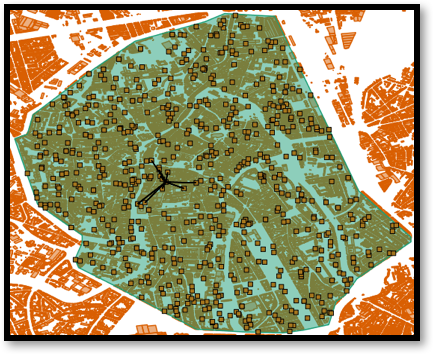
\includegraphics[width=\linewidth]{../images/connectionsMap600Users.png}
\endminipage
  \caption{Overview of which users are connected to the \gls{UABS}. The map on the left is for 50 active users while the map on the right considers 600 active users.}
  \label{fig:connectionMap}
\end{figure}

\subsection{Unlimited Number of UABSs}
\subsubsection{Variable Flying Height}
The same cases as in the previous scenario are investigated. Only now, an unlimited number of \gls{UABS}s is available.
The results prove that the different optimization strategies work as intended.
\gls{PwrC Opt} networks have indeed a lower power consumption but therefore result in higher electromagnetic radiation.
On the other hand, an \gls{Exp Opt} network will reduce the electromagnetic exposure by using more \gls{UAV}s and thence also increase the network's
power consumption.
This conclusion was already made in \cite{J1} and is supported by these results.
\begin{figure}[h!]
  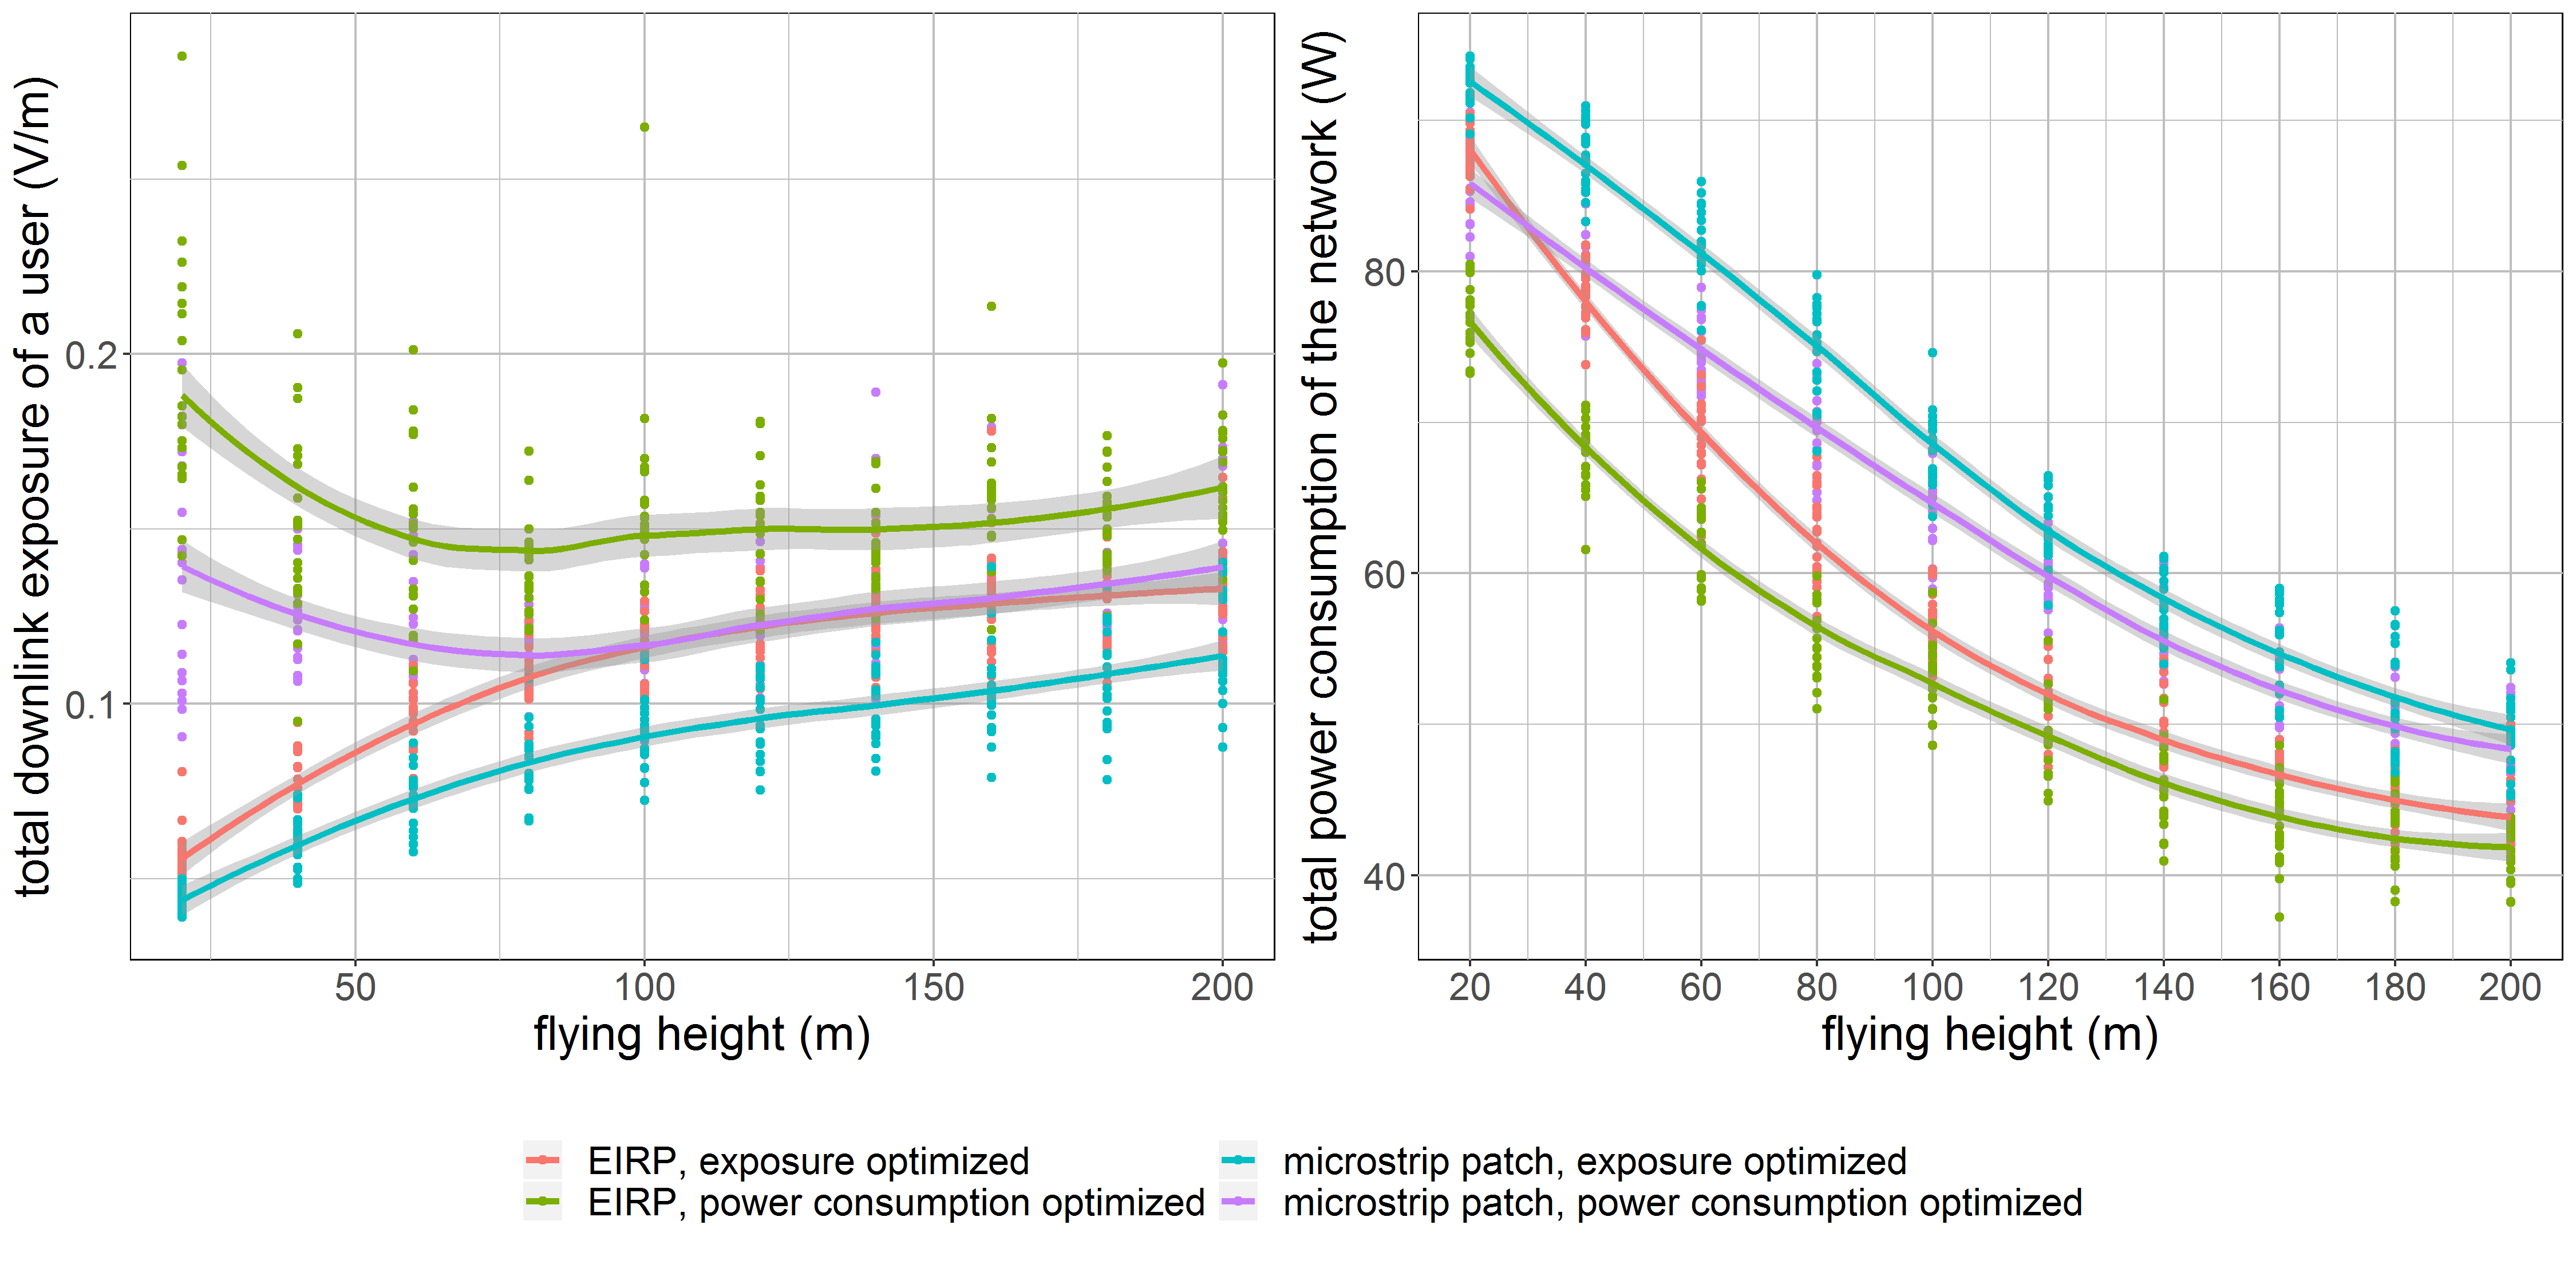
\includegraphics[width=\linewidth]{../results/s3/fhvsdlAndPc.png}
  \caption{These two figures show how the flying height influences the downlink electromagnetic radiation of the average user (left) and 
  power consumption of the entire network (right) for an unlimited number of drones.}
  \label{fig:s3a_dlAndPc}
\end{figure}

The exposure in figure \ref{fig:s3a_dlAndPc} shows that an \gls{Exp Opt} network increases logarithmically while the \gls{PwrC Opt} network rather 
has a concave relationship with the flying height, and has its lowest point at around 70 metres.

At a flying height of 20 m, the \gls{Exp Opt} network has on average 220 to 224 \gls{UABS}s. That is (almost) one \gls{UABS} for each user
so it is logical that the electromagnetic exposure is very low.
The number of \gls{UAV}s in a \gls{PwrC Opt} network is much less in order 
to save energy but it is still able to achieve the same percentage of coverage.
This is done by increasing the radiation so the cover radius would become larger.
The results further show that the network profits from increasing the flying altitude. Not only
less \gls{UAV}s are needed but also the power consumption is lower. Both can be explained by the
lower path loss when UABSs fly higher. 

Figure \ref{fig:s3a_fourSourcesMatrix} shows how each source contributes to the total \gls{SAR}.
A first consequence of higher flying altitudes is the increase in electromagnetic radiation from the user's own device; a behaviour also explained in the first scenario.
A second  consequence is that also 
 the exposure from `other \gls{UABS}s' increases, caused by lower path loss from less obstructing buildings.
The figures from \ref{fig:s3a_fourSourcesMatrix} further also clearly show that this increase 
in electromagnetic radiation will be less for a microstrip patch antenna. The reason behind this is that energy 
will be more focussed towards the ground and there is less sideways radiation because of attenuation.

\begin{figure}[h!]
  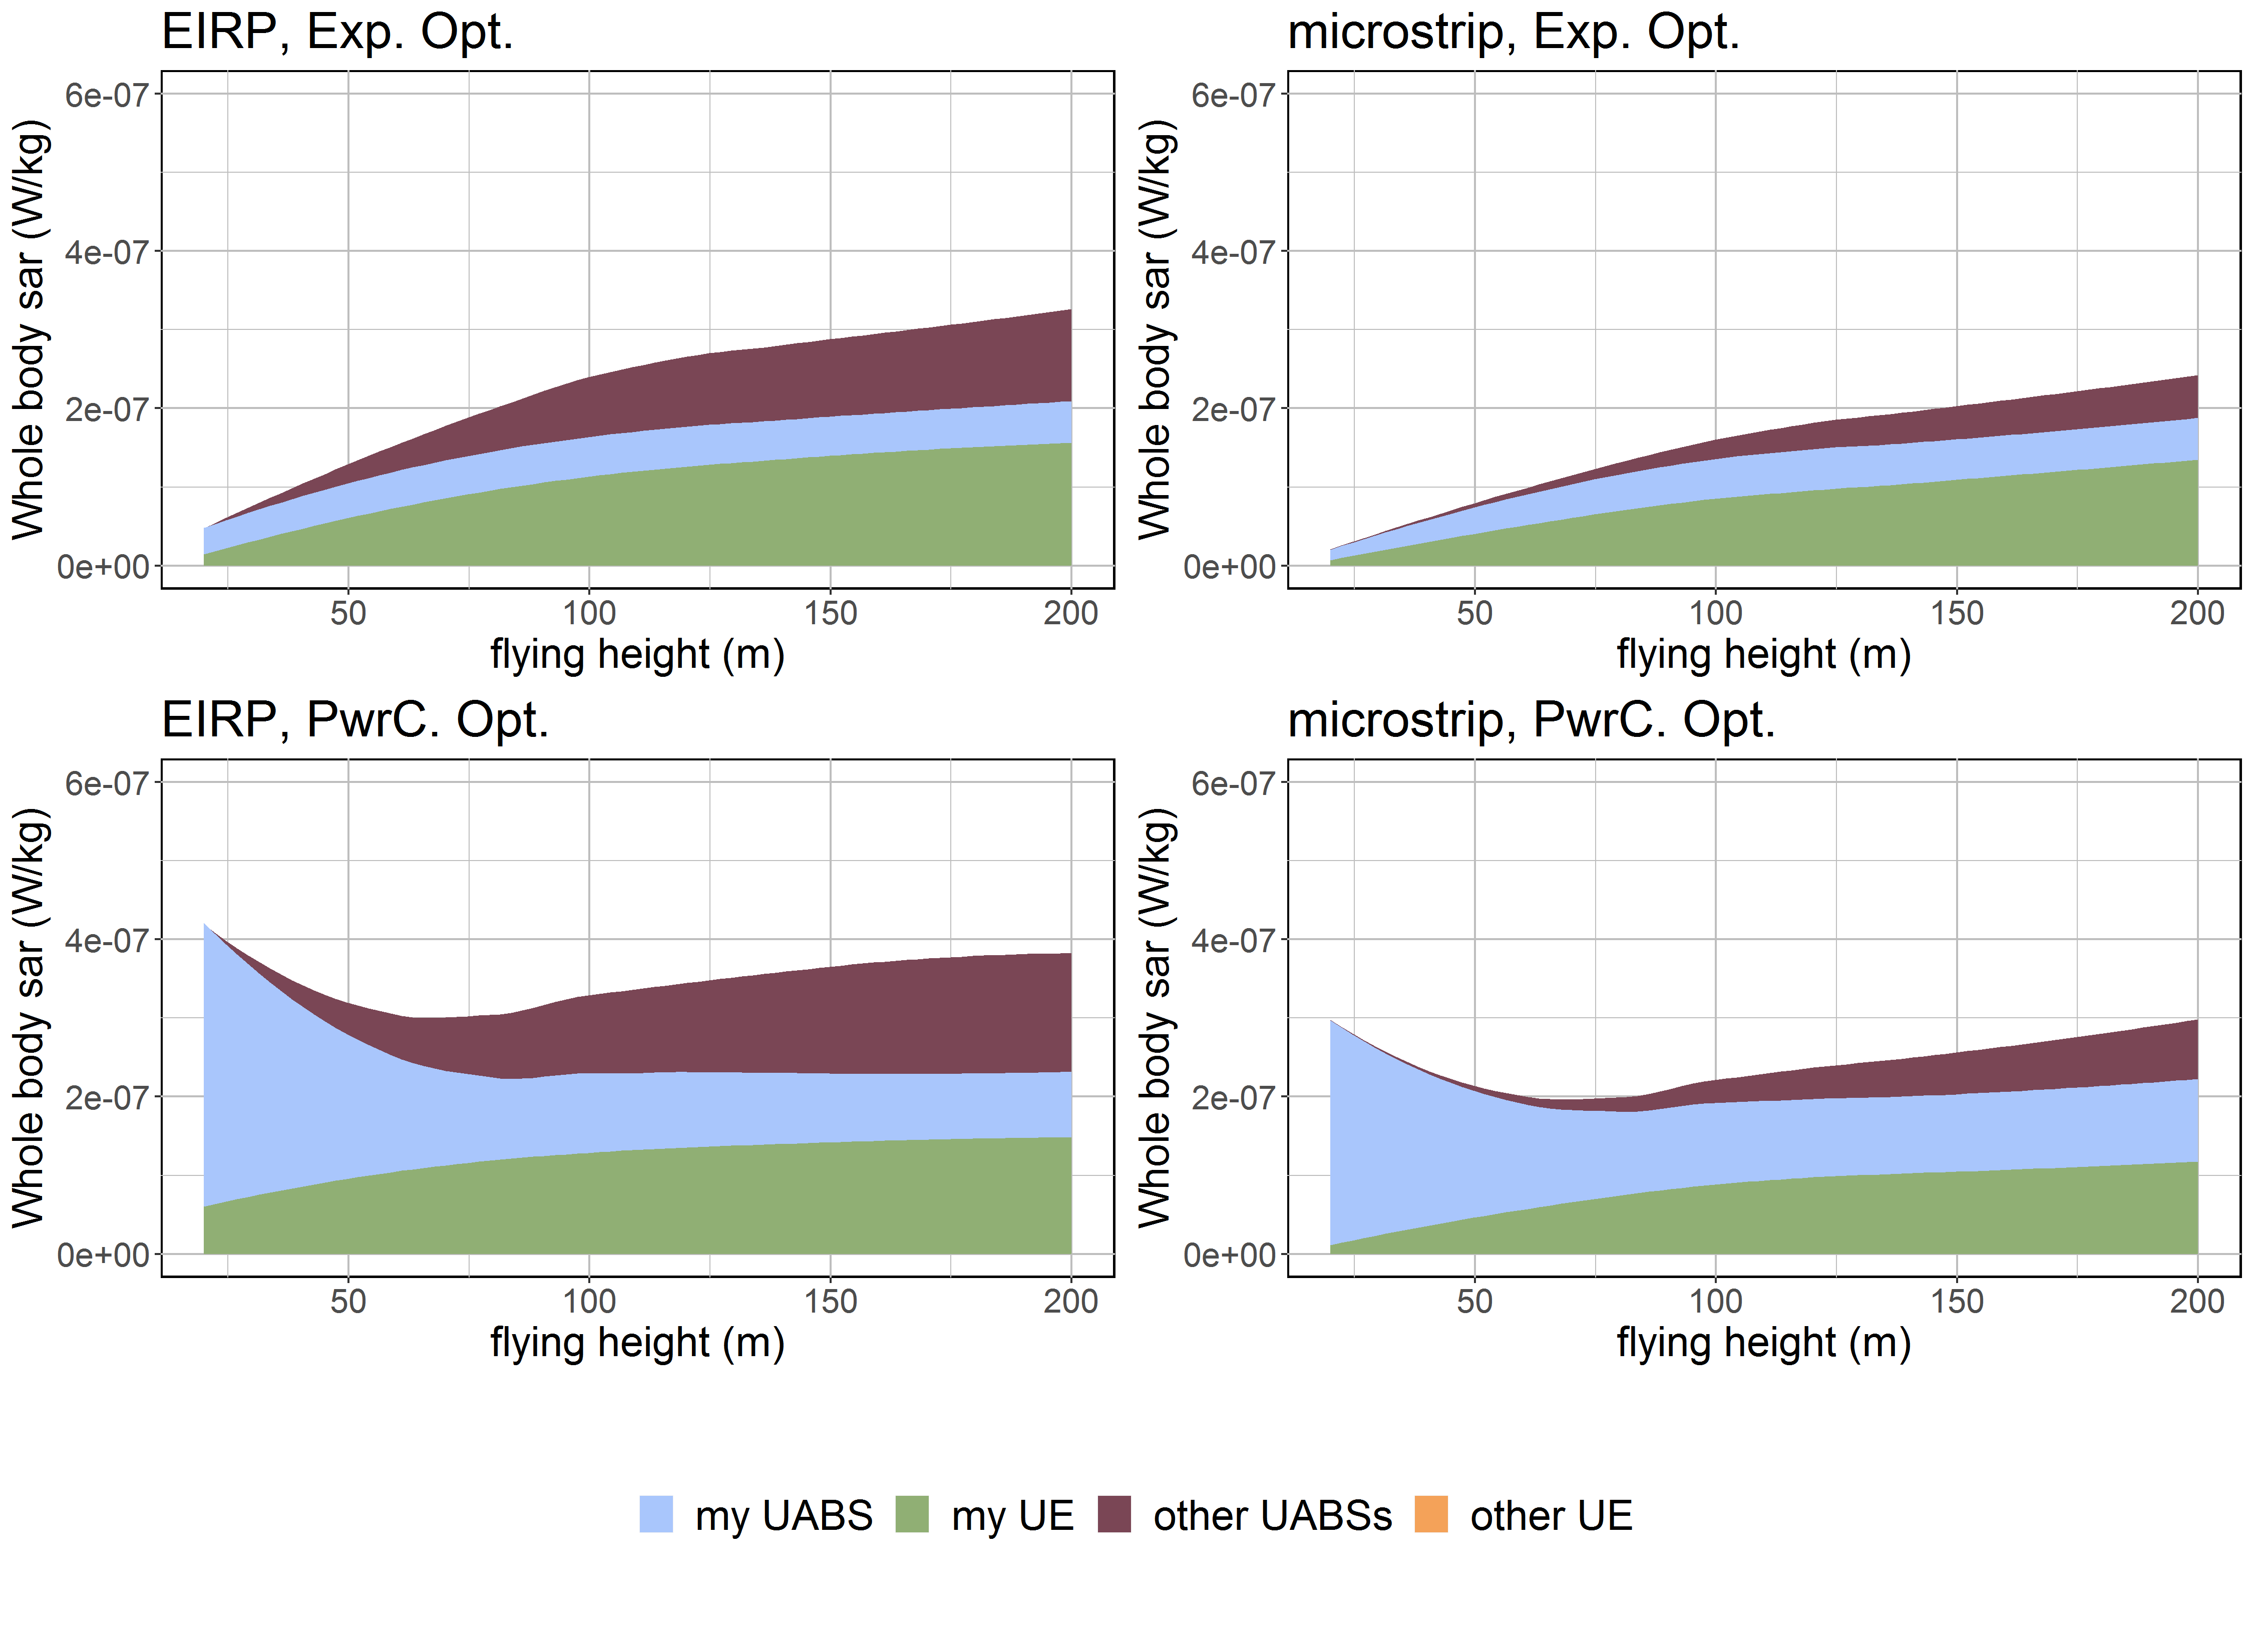
\includegraphics[width=\linewidth]{../results/s3/fhFourSources.png}
  \caption{Each chart corresponds with one of the four possible configurations. The contribution of each source towards the total 
  \gls{SAR} for a varying flying height is shown.}
  \label{fig:s3a_fourSourcesMatrix}
\end{figure}

\subsubsection{Variable Number of Users}
When the flying height of the \gls{UABS}s is fixed to 100 metres and the density of the population increases, also 
the number of required \gls{UAV}s increases in order to reach a 100 \% coverage.
Figure \ref{fig:s3b_dlAndPC} shows that when the number of \gls{UABS}s and users increases, 
also the electromagnetic exposure and power consumption increases.
Once again, the EIRP antenna in a power consumption network has the highest exposure for the lowest power consumption
and a microstrip patch antenna in an \gls{Exp Opt} network the lowest exposure for the highest power consumption.
The two other combinations are in the middle and behave very similar.

\begin{figure}[h!]
  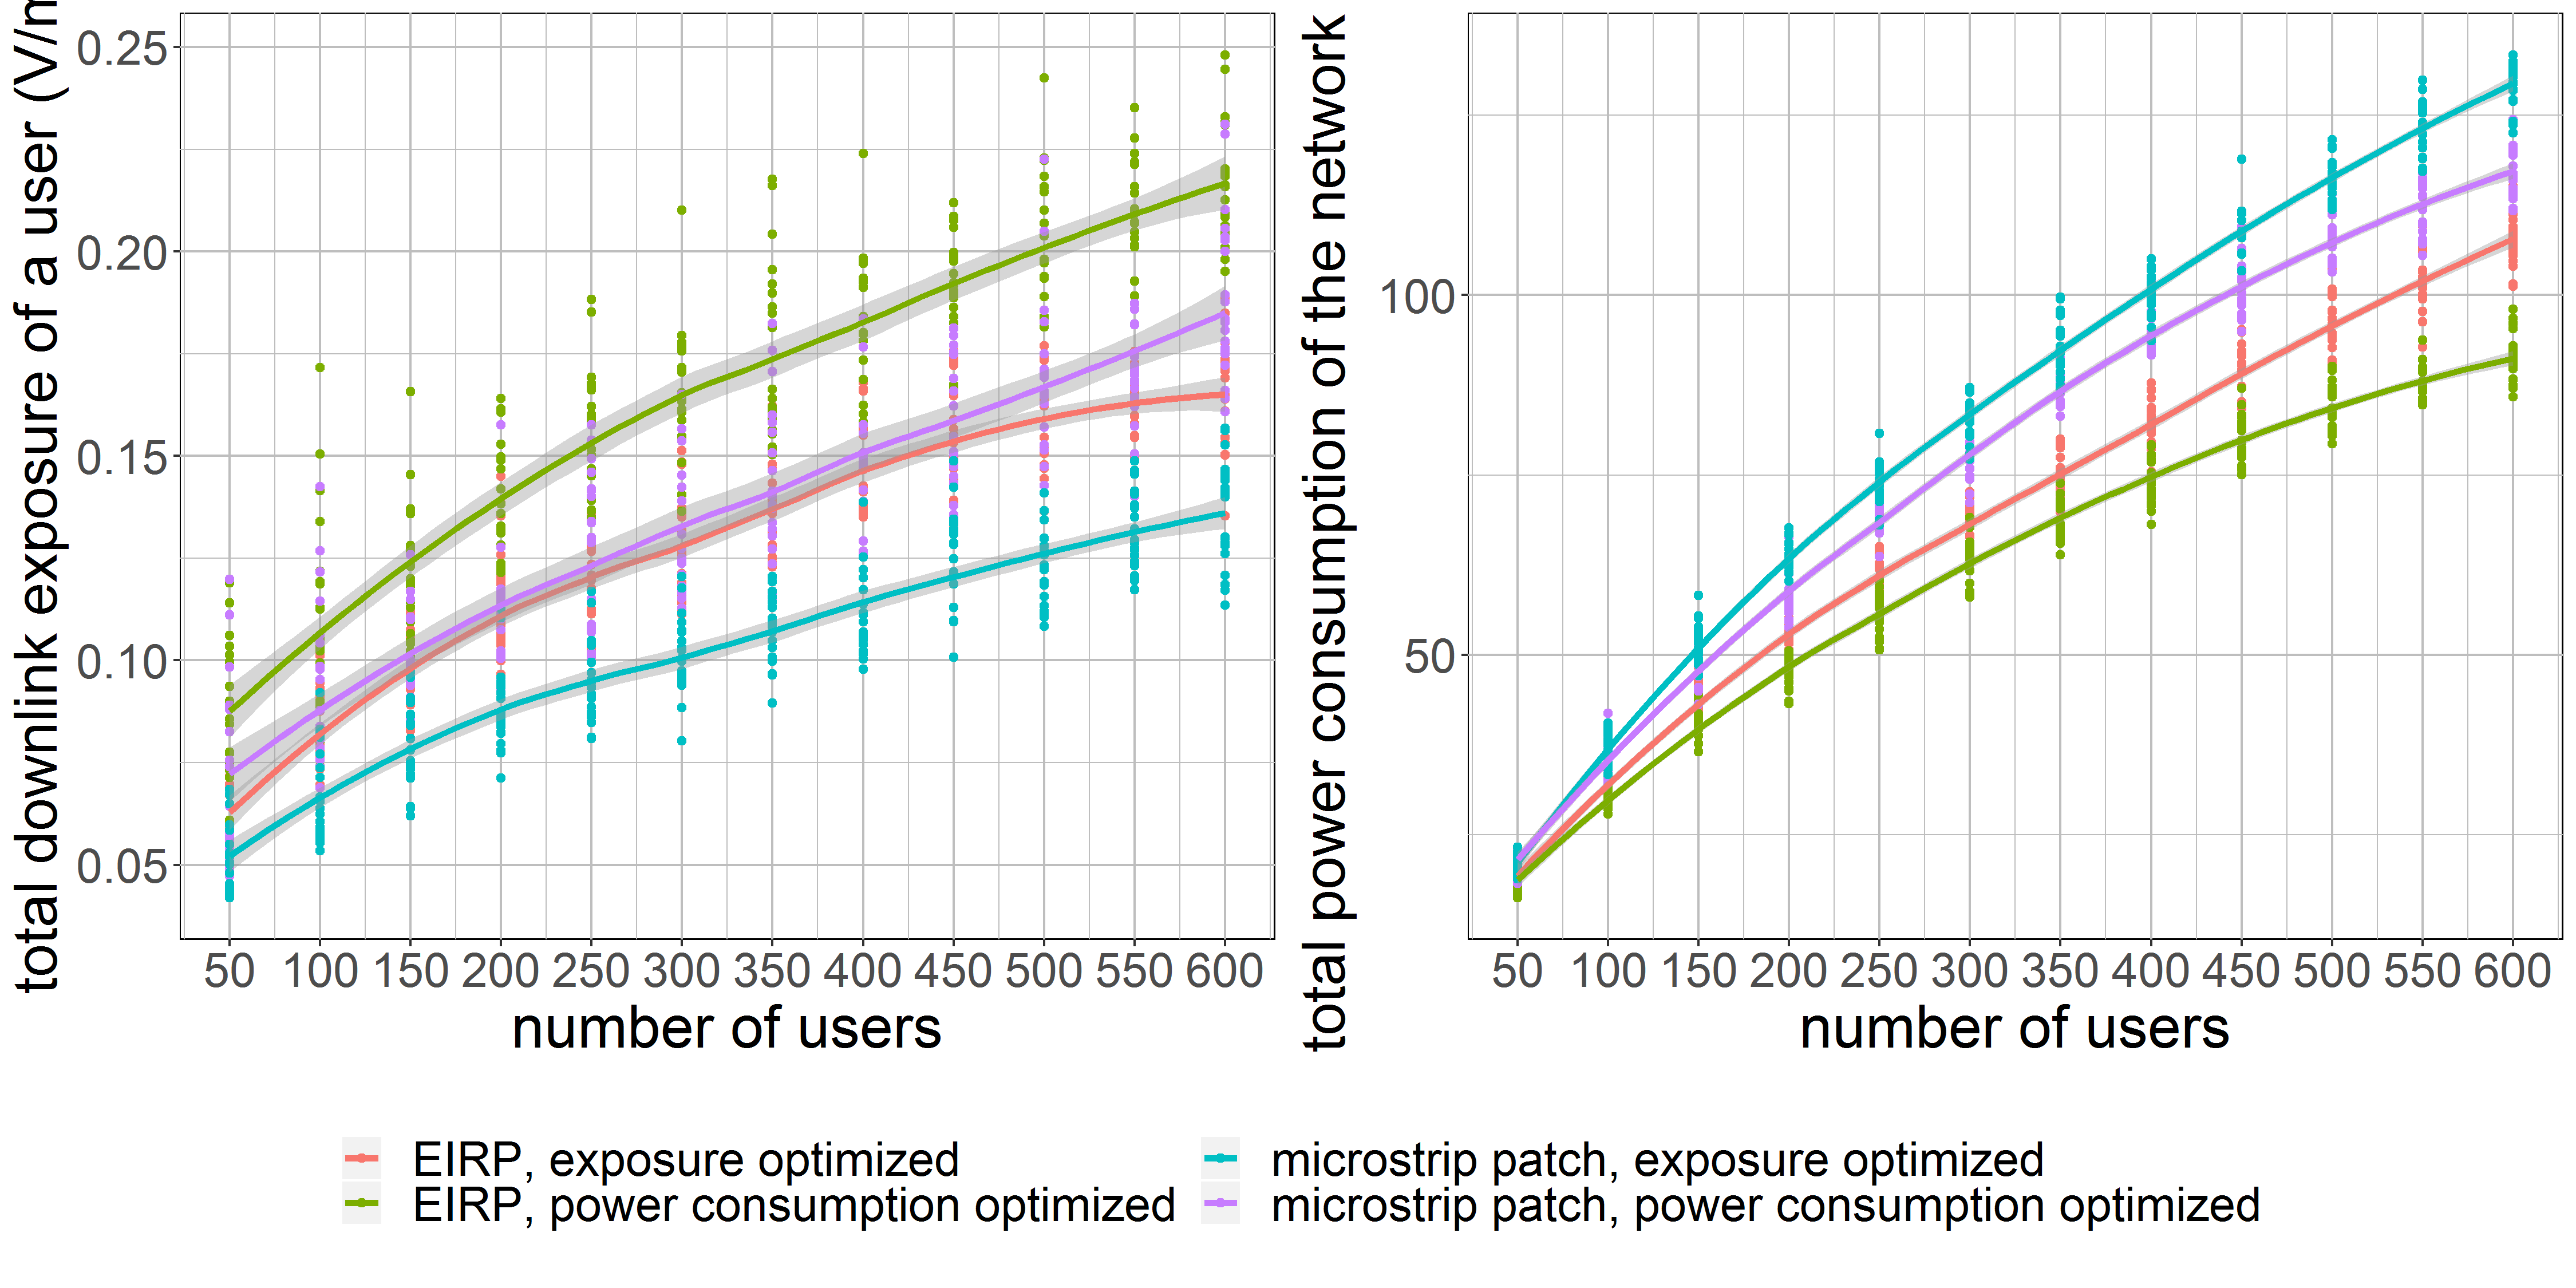
\includegraphics[width=\linewidth]{../results/s3/uvsdlAndPc.png}
  \caption{These two figures show how the number of users influences the downlink electromagnetic radiation of the average user (left) and 
  power consumption of the entire network (right) for an unlimited number of drones.}
  \label{fig:s3b_dlAndPC}
\end{figure}

When looking at the different contributions to the total \gls{SAR} in figure \ref{fig:s3b_fourSourcesMatrix}, 
we see that the weighted average 
\gls{SAR} from the users' own device and from the serving \gls{UABS} remains constant. The flying altitude is always the same so 
also the required energy to cover that distance will remain the same. 
The only \gls{SAR} values that increase are the \gls{DL} \gls{SAR} from other \gls{UABS}s and the \gls{UL} \gls{SAR} 
from other \gls{UE}. 
When more users come online, also more \gls{UAV}s will be radiating. The electromagnetic
radiation will thus increase for both types of sources. Moreover, there is very little path loss at this flying altitude since it 
is higher than the average building.

\begin{figure}[h!]
  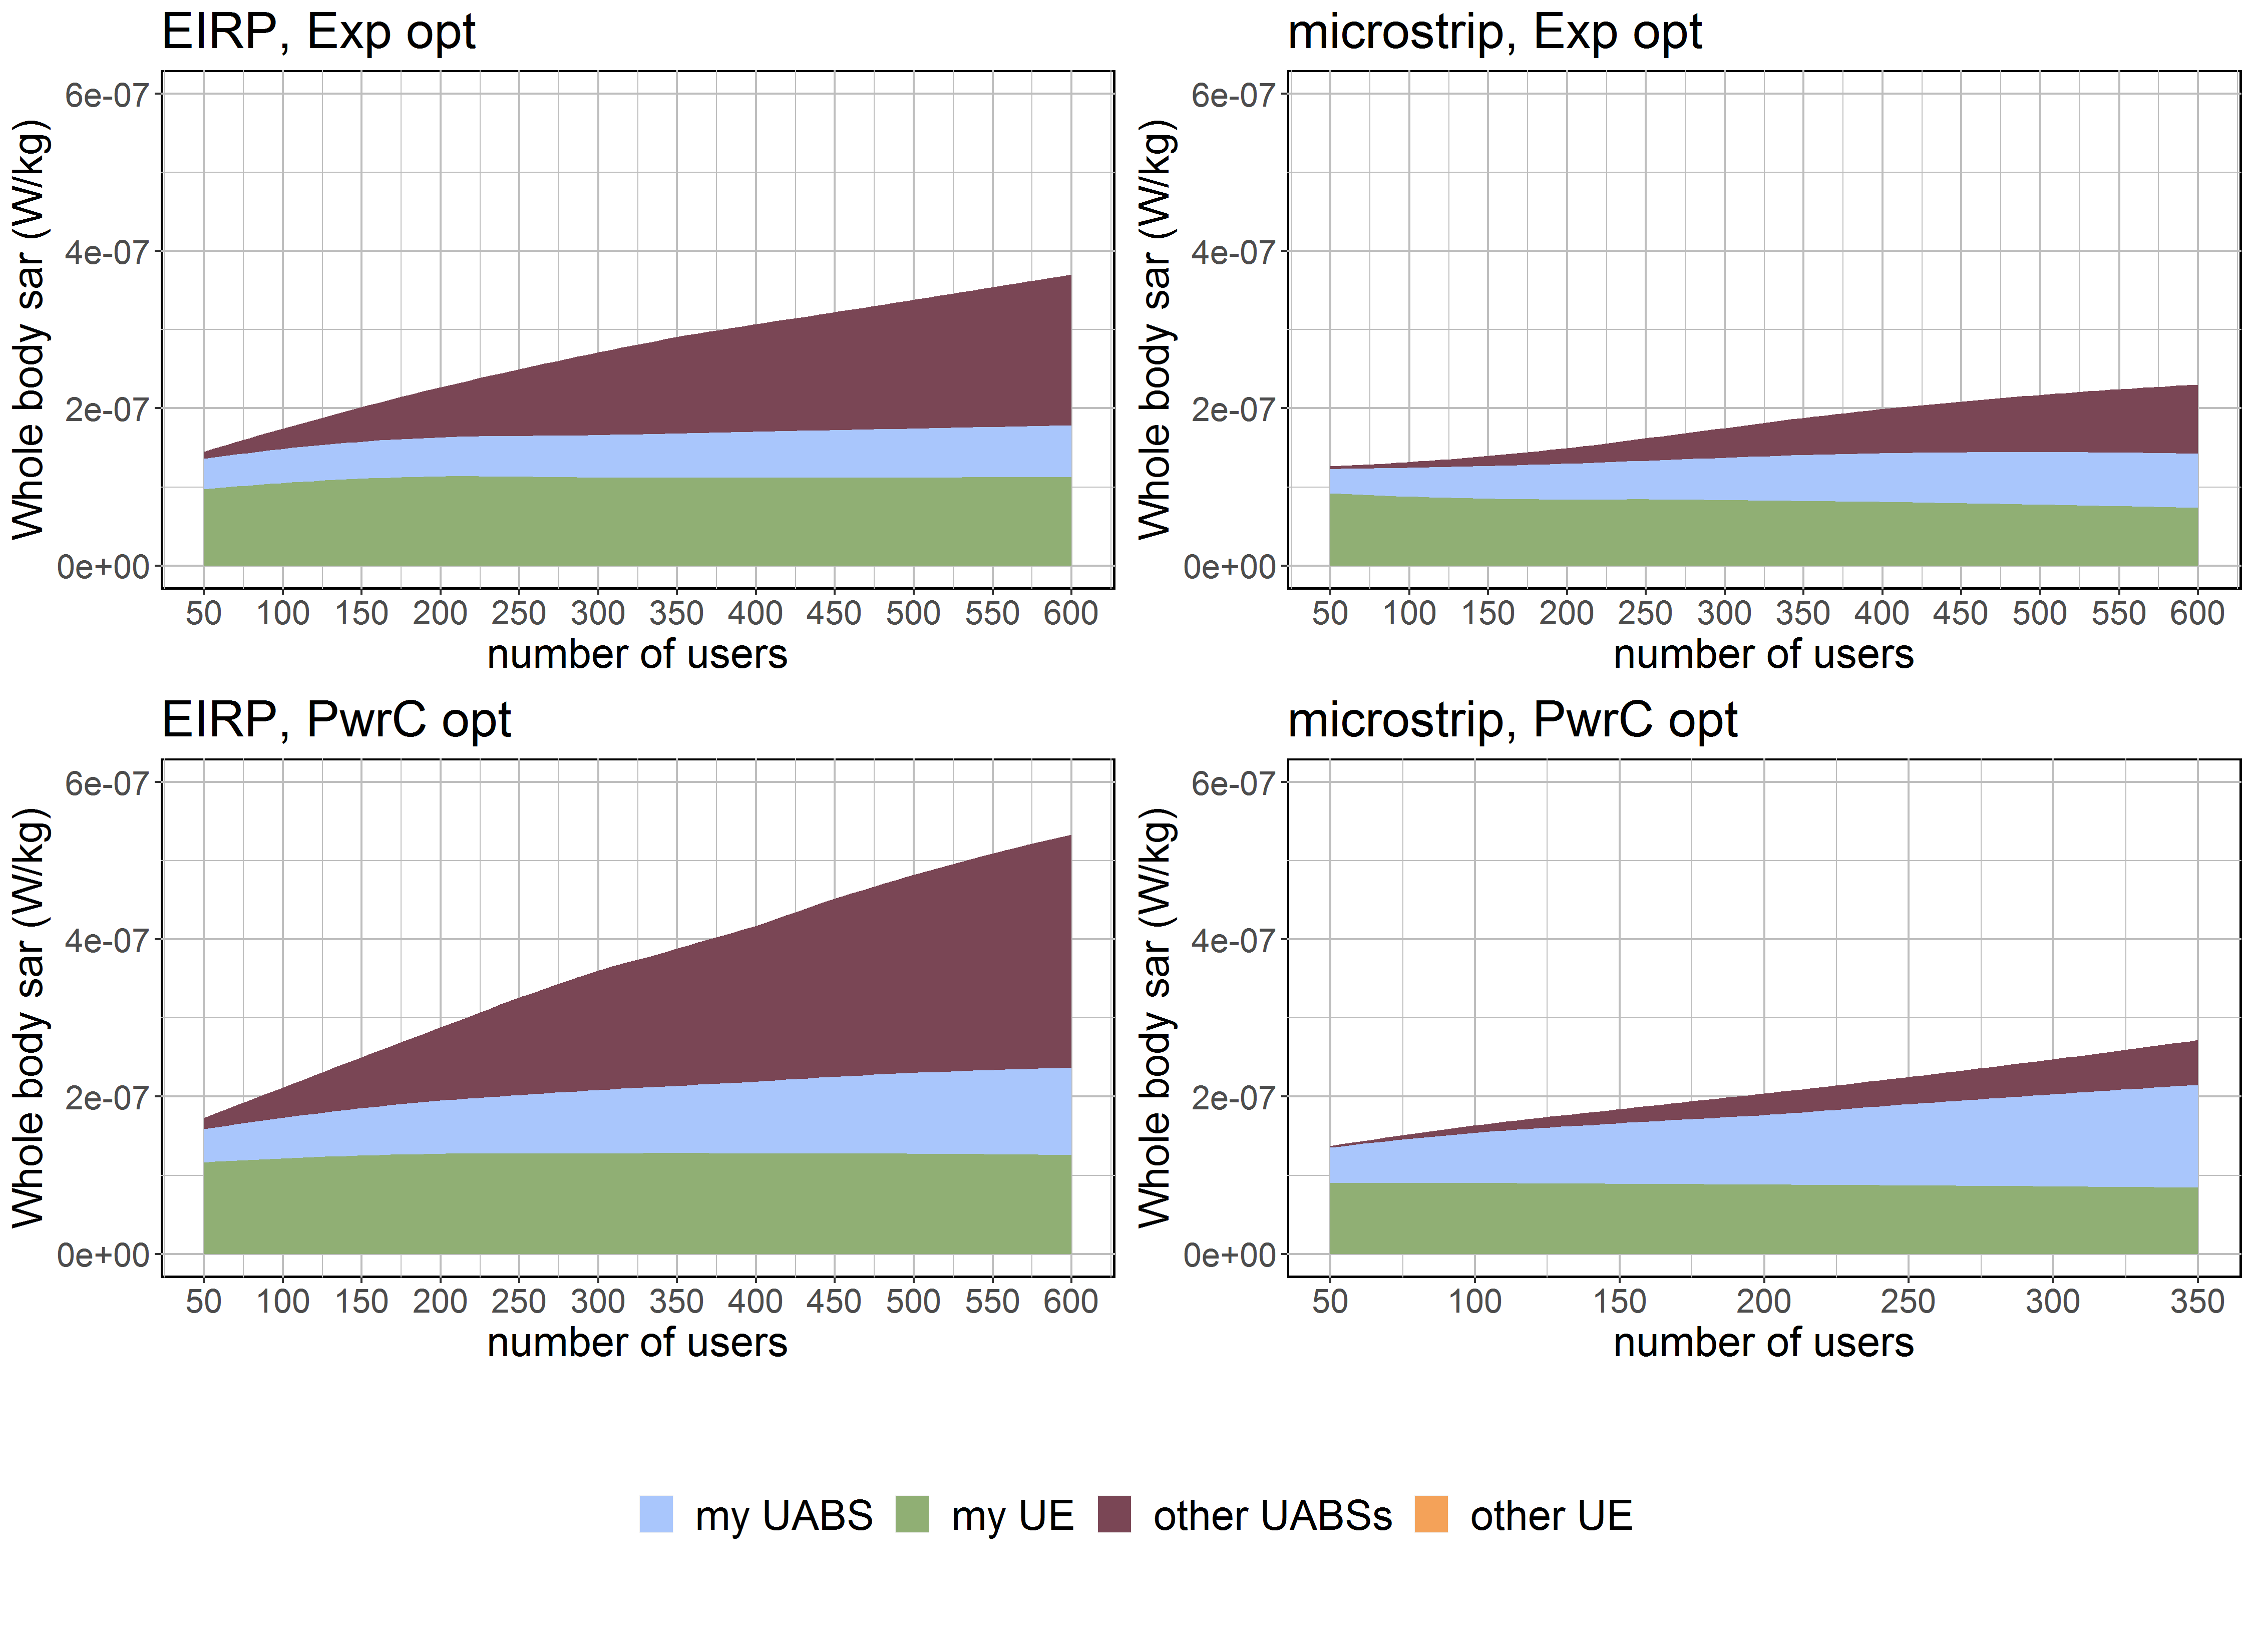
\includegraphics[width=\linewidth]{../results/s3/uFourSources.png}
  \caption{Each chart corresponds with one of the four possible configurations. The contribution of each source towards the total 
  \gls{SAR} for a varying number of users shown.}
  \label{fig:s3b_fourSourcesMatrix}
\end{figure}

\section{Conclusion}
%How can a UABS network be optimized to minimize global exposure or overall power consumption? 
Literature showed that a network can be optimized towards either the power consumption of the entire network 
or the electromagnetic exposure of the average user using a fitness function \cite{J1}.
However, the fitness function should be used with care considering that \gls{UABS}s can be placed anywhere as opposed to 
the transmission towers from \cite{J1} who have a predetermined position. 
In an \gls{Exp Opt} network, this causes a lot of users to get a \gls{UABS} all by 
themselves because this is the best approach to minimize exposure.
A \gls{PwrC Opt} network on the other hand will try to limit the number of drones 
in order to save energy. 
So as a rule of thumb: an \gls{Exp Opt} network will result in a lot of low powered devices (increasing the overall power consumption)
while a \gls{PwrC Opt} network results in a few high powered devices (increasing the exposure of the average user).
If the goal is to remain in the air for a longer period of time, an \gls{Exp Opt} network is recommended because the power consumption of 
an individual \gls{UABS} is lower.
On the other hand, a \gls{PwrC Opt} network is cheaper because less drones are involved. 
Moreover, the results show that the electromagnetic radiation in a \gls{PwrC Opt} network (with high powered \gls{UABS}s)
is far below the thresholds enforced by the Flemish government.

The user's main sources of exposure are the user's own device and the \gls{UABS} who is serving him, followed by all
other \gls{UABS}s in the network. 
When the population increases, there is not only more radiation from \gls{UE} but also 
from more \gls{UABS}s that are serving the other users.
The exposure from other people's \gls{UE} is so low that it can be neglected.
An \gls{Exp Opt} network will limit the total exposure mainly by trying to reduce the exposure from other \gls{UABS}s.

%1)	How does the network behave differently after the introduction of a realistic antenna?
A directional microstrip patch antenna is introduced because it gives several advantages compared to omnidirectional antennae.
Directional antennae are able to focus their energy there where it is needed, namely towards the ground. Microstrip patch antennae 
further benefit from their thin and lightweight design. The performance 
of this directional microstrip patch antenna has been compared to a 
fictional \gls{isotropicradiator}.
This \gls{isotropicradiator} has higher exposure and coverage for less power, compared to realistic antennae like microstrip patch antennae
because of the absence of attenuation, and can hypothetically be compared with an antenna with a very big aperture angle.
This type of antenna can achieve the same coverage with less
resources like power and number of drones. 
A microstrip patch antenna with a more limited aperture angle of \ang{90} requires more resources but 
causes less sideways radiation. So the exposure from other \gls{UABS}s will be way less.

\begin{figure}[h!]
  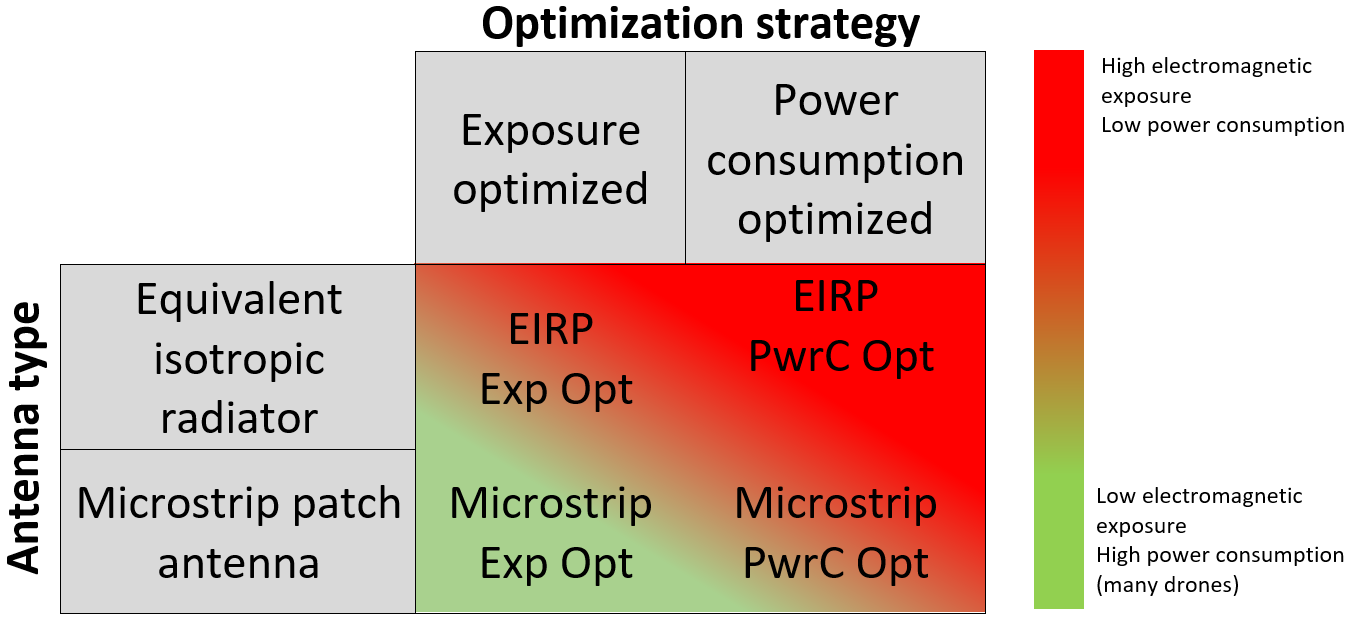
\includegraphics[width=\linewidth]{fourCasesMatrixSol.png}
  \caption{Matrix with the four possible configurations, colour-coded based on the results.}
  \label{fig:resultIllustration}
\end{figure}

Remarkable is that an \gls{EIRP} \gls{Exp Opt} network behaves very similar to a microstrip \gls{PwrC Opt} network as shown 
in figure \ref{fig:resultIllustration}.
This results in the best of both worlds. 
The microstrip patch antenna will generate less electromagnetic radiation by design and
 the power consumption optimization reduces the number of required drones and power. A microstrip patch antenna with an aperture 
 angle of \ang{90} is considered as a good solution but if budget is limited, an antenna with a larger aperture angle 
 would further reduce cost without interfering with the Flemish legislation regarding electromagnetic exposure.

The electromagnetic radiation of an \gls{Exp Opt} network increases with higher flying altitudes.
Around 80 metres, the exposure from the  user's device surpasses the exposure from the serving \gls{UABS}.
On the other hand, a \gls{PwrC Opt} network shows that the lowest exposure is measured around 70 to 80 metres.
Further, the results also show that the number of required drones decreases when the flying height becomes larger; a conclusion that was also made in \cite{J2}.
When also considering the results from \cite{U1} where a flying altitude from 
80 metres is suggested for an optimal access and backhaul connectivity, a flying height 
of 80 metres is also here proposed for the city centre of Ghent.

In short, a \gls{PwrC Opt} network is proposed with a fixed flying height of 80 metres. A microstrip patch 
antenna with a sufficiently large aperture angle is a good starting point. However, different antenna configurations should 
be investigated.

\section*{Acknowledgement}
Special thanks to the WAVES research group at Ghent University for providing 
access to their capacity based deployment tool and therefore making this research possible.

\bibliographystyle{ieeetr}
\bibliography{referenties}


\end{document}
